\documentclass{article}

\usepackage{amsmath}
\usepackage{amssymb}
\usepackage{amsthm}
\usepackage{enumerate}
\usepackage{relsize}
\usepackage{algorithm}
\usepackage{algpseudocode}
\usepackage{parskip}
\usepackage{graphicx}
\usepackage{cite}
\usepackage{xcolor}
\usepackage{caption}
\usepackage{float}
\graphicspath{{images/}}

\usepackage[
  top    = 2.75cm,
  bottom = 3.00cm,
  left   = 2.50cm,
  right  = 2.50cm
]{geometry}

\captionsetup{font=footnotesize,justification=justified,margin=2cm}

\algnewcommand\algorithmicinput{\textbf{Input:}}
\algnewcommand\algorithmicoutput{\textbf{Output:}}
\algnewcommand\algorithmicsideeffect{\textbf{Side Effect:}}
\algnewcommand\Input{\item[\algorithmicinput]}
\algnewcommand\Output{\item[\algorithmicoutput]}
\algnewcommand\SideEffect{\item[\algorithmicsideeffect]}
\algnewcommand{\IIf}[1]{\State\algorithmicif\ #1\ \algorithmicthen}
\algnewcommand{\IIEf}[2]{\State\algorithmicif\ #1\ \algorithmicthen\ #2\ \algorithmicelse}
\newcommand{\compatible}{\smile}
\newcommand{\leafset}{\Lambda}
\newcommand{\weight}{\omega}
\newcommand{\TA}{T_\alpha}
\newcommand{\TB}{T_\beta}

\title{A Faster Construction of Frequency Difference Consensus Trees\\CG4001 Interim Report}
\author{Varun Gupta\\A0147924X}

\newtheorem{incompatibility}{Lemma}
\newtheorem{freqdiffruntimecomponents}[incompatibility]{Corollary}
\newtheorem{lca}[incompatibility]{Lemma}
\newtheorem{linearrmq}[incompatibility]{Lemma}
\newtheorem{mergetrees}[incompatibility]{Lemma}
\newtheorem{cfddatastructure}[incompatibility]{Lemma}
\newtheorem{cfdquery}[incompatibility]{Lemma}
\newtheorem{rmqdatastructure}[incompatibility]{Lemma}
\newtheorem{rmqquery}[incompatibility]{Theorem}
\newtheorem{assocnode}[incompatibility]{Lemma}
\newtheorem{labelclusterscorrectness}[incompatibility]{Lemma}
\newtheorem{labelclustersidbounds}[incompatibility]{Lemma}
\newtheorem{labelclustersruntime}[incompatibility]{Lemma}
\newtheorem{weightingruntime}[incompatibility]{Lemma}
\newtheorem{computerootsofsubtreesruntime}[incompatibility]{Lemma}
\newtheorem{maintainingcounter}[incompatibility]{Lemma}
\newtheorem{incompatibilityrootsofsubtrees}[incompatibility]{Lemma}
\newtheorem{incompatibilityrecursive}[incompatibility]{Lemma}
\newtheorem{filterclustersruntime}[incompatibility]{Lemma}
\newtheorem{freqdiffruntime}[incompatibility]{Theorem}

\begin{document}
    \maketitle

    \begin{abstract}
        This report presents a new deterministic algorithm for constructing a frequency difference consensus tree. Given $k$ phylogenetic trees with identical leaf label sets of size $n$, this algorithm constructs the frequency difference tree in $O(kn\,log\,n)$ time, bettering the previously best known time of $O(kn\,log^2n)$.
    \end{abstract}

    \section{Introduction}
    \label{sec:introduction}

    A \textit{taxon} (pl. taxa) is a group of organisms that taxonomists classify as a single unit, such as \textit{homo sapiens}. These come together to give a \textit{rooted phylogenetic tree}, which presents the evolutionary relationships between various taxa in a hierarchical manner. Each leaf in this tree represents a taxon. An internal node then represents the common ancestor of a subgroup of the taxa shown in the entire tree. Children of each node split the group rooted at that node into smaller ones. A subgroup of taxa that are descendants of some common ancestor is called a \textit{clade}, i.e. a clade is the leaf set of any node in a phylogenetic tree.

    We often obtain multiple phylogenetic trees from biological datasets. These trees may be produced from different datasets or from a single dataset using techniques like maximum parsimony that yield a number of candidate trees \cite{bryant1997hunting}. This motivates the concept of a \textit{consensus tree}, which reconciles many phylogenetic trees by summarising the branching information contained in each into a single tree. Consensus trees are also useful in determining which clades have strong suppport within the input trees \cite{felsenstein2004inferring}.

    A variety of techniques of constructing a consensus tree from a set of phylogenetic trees have been developed over the last half century, starting with the Adams consensus tree \cite{adams1972consensus} in 1972. There is a strong motivation for the development of different types of consensus trees since they each have their own benefits and drawbacks. Some of these techniques are summarised in \S 6.2 of \cite{bryant1997hunting} and a comparative analysis can be found in \cite{bryant2003classification}. We illustrate some techniques here. The \textit{strict consensus tree} \cite{sokal1981taxonomic} only keeps those clades that occur in all the input trees. While easily reconstructed and interpreted, it can discard a lot of potentially important information if there is a lot of disagreement between the various trees. The \textit{majority rule consensus tree} \cite{margush1981consensusn} is a generalisation of the previous, allowing all clades that occur in a majority of the trees. Holder et al. \cite{holder2008justification} showed that these trees are optimal given a certain context.

    This article studies a specific type of consensus tree, known as the \textit{frequency difference consensus tree} \cite{goloboff2003improvements}. The \textit{frequency difference consensus tree} (abbreviated henceforth as FDCT) further generalises the \textit{majority rule consensus tree}, keeping every clade that occurs in more trees than the most frequent clade that contradicts it (the concept of contradiction is formalized in Subsection~\ref{subsec:def}). The FDCT is motivated by a desire to design an effective criterion for determining which clades are strongly supported within a set of trees. As set out in \cite{goloboff2003improvements}, although the \textit{majority rule consensus tree} includes a clade that is supported by 60\% of a set of trees and contradicted by 40\% of them, it does not include a clade supported by 40\% of the trees but not contradicted by any of them. A possible resolution to this is to define strongly supported clades as those with greater frequency than all clades incompatible with them. These are called frequency difference clades and all of these are included in the FDCT.

    Dong et al. \cite{dong2010majority} provided a comparison of the FDCT and a few other types of consensus trees. Barrett et al. \cite{barrett2013plastid} employed the idea of using frequency difference as a measure of clade support while analysing angiosperm phylogeny and commented ``[the] frequency difference metric ... is particularly useful for assessing support when it is not overwhelmingly in favour of one particular topology, and should be especially useful in phylogenomic analyses in general, where hundreds or thousands of characters may contribute to branch support''. Steel and Velasco \cite{steel2014axiomatic} investigated a generalisation of the FDCT to \textit{supertrees}, i.e. consensus trees built from input trees that do not necessarily have the same leaf sets. They show that, unlike some other popular techniques, the FDCT definition easily generalises to a viable supertree definition and conclude that the FDCT is ``worthy of more widespread usage and serious study''. Given that the FDCT and the frequency difference measure have been utilised in various studies over the years \cite{garcia2014testing,barrett2013plastid,molineri2010cladistic,molineri2013phylogeny,molineri2015phylogeny,lindqvist2006molecular,han2014new} and keeping in mind the favourable opinions above, we set out to improve upon the best known deterministic algorithm for reconstructing the FDCT of a set of trees.

    \subsection{Definitions and Notation}
    \label{subsec:def}

    We define a rooted phylogenetic tree to be a rooted, leaf-labelled tree where every internal node has 2 or more children and every leaf has a different label. Henceforth, we will simply refer to these as trees. Let $T$ be some tree. The set of nodes of $T$ is denoted by $V(T)$. For any node $u \in V(T)$, the \textit{parent} of $u$ (if it exists) is represented by $parent^T(u)$ and the set of its \textit{children} is represented by $children^T(u)$. The \textit{depth} of $u$, denoted by $depth^T(u)$ is the number of nodes that are its proper ancestors. A node that is \textit{shallower} than another has a smaller depth value. Let $\leafset^T$ be the set of leaf labels of $T$. Non-empty subsets of $\leafset^T$ are called \textit{clusters} (we use the term clusters instead of clades for consistency with recent literature). Clusters with cardinality $1$ or $|\leafset^T|$ are \textit{trivial clusters}. For any node $u \in V(T)$, $T[u]$ is the subtree of $T$ rooted at $u$ and $\leafset^T(u)$ is the leafset of $T[u]$, called the cluster \textit{associated} with $u$. For example, in Figure~\ref{fig:freqdiff}, the node labelled by $2$ in $T_1$ has the cluster $\{a, b\}$ associated with it. The \textit{cluster collection} of $T$, $\mathcal{C}(T)$ is the set $\bigcup_{u \in V(T) - \{root(T)\} - \leafset^T} {\leafset^T(u)}$, i.e. a set containing all non-trivial clusters in $T$. For example, the cluster collection of $T_2$ in Figure~\ref{fig:freqdiff} is $\{\{b, c\}, \{a, b, c\}, \{d, e\}\}$. Any cluster $C \subseteq \leafset(T)$ \textit{occurs} in $T$ iff $C \in \mathcal{C(T)}$. Also, for any nodes $u, v \in V(T)$, denote the lowest common ancestor of $u$ and $v$ in $T$ by $lca^T(u, v)$. Further, for any non-empty set of nodes $U \subseteq V(T)$, denote the lowest common ancestor of all these nodes in $T$ by $lca^T(U)$.

    Any two clusters $C_1, C_2 \subseteq \leafset(T)$ are said to be \textit{compatible}, denoted as $C_1 \compatible C_2$, iff $C_1 \subseteq C_2$ or $C_2 \subseteq C_1$ or $C_1 \cap C_2 = \emptyset$. If $C_1$ and $C_2$ satisfy none of the preceding properties, then they are said to be \textit{incompatible} (referred to as \textit{contradiction} in Section~\ref{sec:introduction}), denoted as $C_1 \not\compatible C_2$. Similarly, given trees $T_1$ and $T_2$ with identical leaf sets, and nodes $u \in V(T_1)$, $v \in V(T_2)$, we say $u$ is compatible with $v$, denoted as $u \compatible v$, if the clusters associated with $u$ and $v$ are compatible. For example (referring to Figure~\ref{fig:freqdiff}), let $u$ be the node in $T_1$ associated with the cluster $\{a, b\}$, $v$ the node in $T_2$ associated with $\{a, b, c\}$ and $w$ the node in $T_2$ associated with $\{b, c\}$. Then $u$ and $v$ are compatible since $\leafset^{T_1}(u) \subseteq \leafset^{T_2}(v)$. However, $u$ is incompatible with $w$ since they share $b$ but neither leafset is a subset of the other. We now extend the notion of compatibility to trees. A cluster $C \subseteq \leafset(T)$ is \textit{compatible} with $T$ (denoted as $C \compatible T$) iff for every $C_1 \in \mathcal{C}(T)$, $C \compatible C_1$. Further, two trees $T_1$ and $T_2$ with identical leafsets are \textit{compatible} (denoted as $T_1 \compatible T_2$) iff for every $C \in \mathcal{C}(T_1)$, $C \compatible T_2$, i.e. if every cluster in $T_1$ is compatible with $T_2$. Observe that this also means that every cluster in $T_2$ is compatible with $T_1$. Thus in Figure~\ref{fig:freqdiff}, $T_1$ is incompatible with $T_2$ since the former contains the cluster $\{a, b\}$ which is incompatible with $\{b, c\}$, contained in the latter tree (in fact, it can be checked that all the trees in this figure are incompatible).

    \begin{figure}[h]
        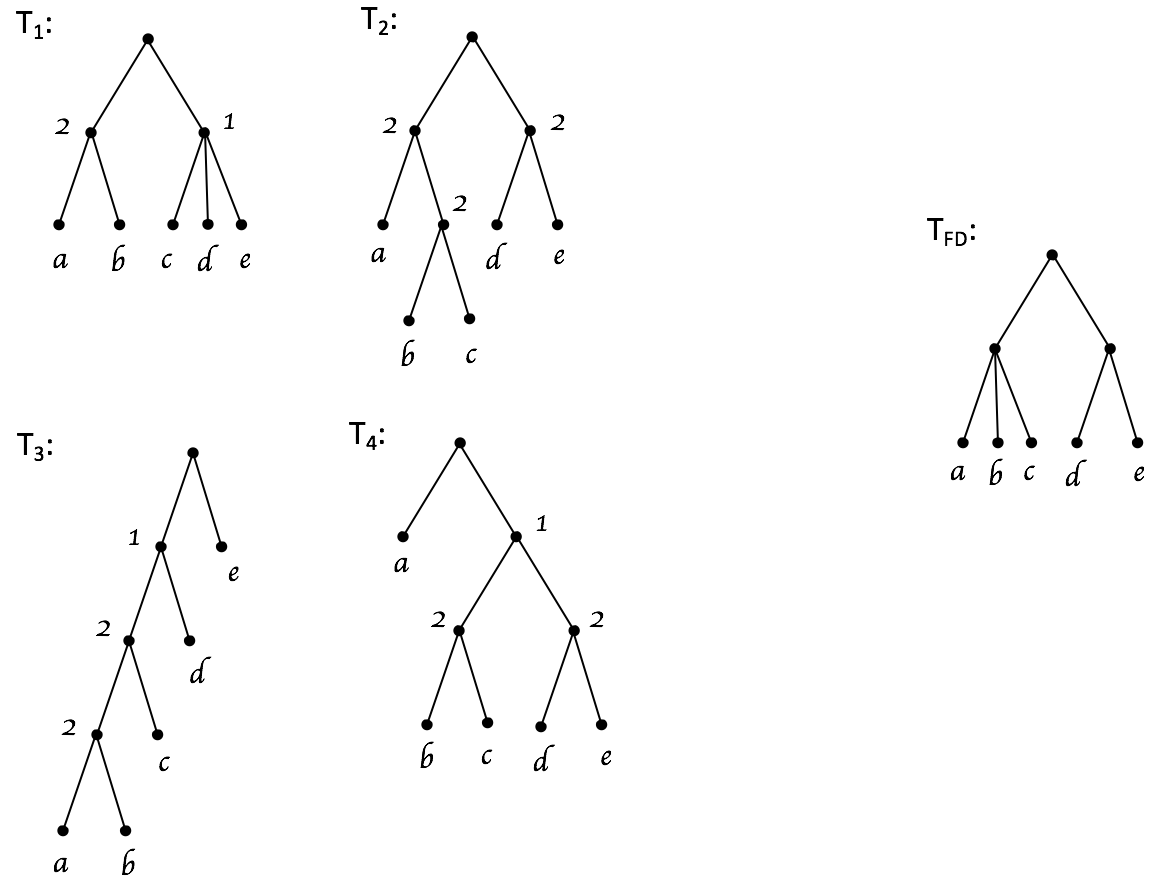
\includegraphics[scale=0.5]{freqdiff}
        \centering
        \caption{Let $\mathcal{S} = \{T_1, T_2, T_3, T_4\}$. $T_{FD}$ is the FDCT of $\mathcal{S}$. The number beside each non-root internal node $u$ indicates the weight of the node, $\weight(u)$, which is the number of occurences of the cluster $\leafset(u)$ in $\mathcal{S}$.}
        \label{fig:freqdiff}
    \end{figure}

    A \textit{frequency difference consensus tree} is defined as follows. Let $\mathcal{S}$ be a set of $k$ trees with identical leaf labels, i.e. $\mathcal{S} = \{T_1, T_2, ..., T_k\}$, where $\leafset(T_1) = \leafset(T_2) = ... = \leafset(T_k) = L$. For any cluster $C \subseteq L$, let weight of $C$, denoted as $\weight(C)$, be $|\{T : T \in \mathcal{S} \text{ and } C \in \mathcal{C}(T)\}|$, i.e. the number of trees in $\mathcal{S}$ which $C$ occurs in. For convenience, we also define, for any tree $T \in \mathcal{S}$, for any node $u \in V(T)$, the weight of $u$, denoted as $\weight(u)$ to be $\weight(\leafset^{T}(u))$. Then the FDCT of $\mathcal{S}$ is the tree $T_{FD}$, where $\mathcal{C}(T_{FD}) = \{C : C \subseteq L \text{ and } \weight(C) > max(\{\weight(C_1) : C_1 \subseteq L \text{ and } C \not\compatible C_1\})\}$. Thus $T_{FD}$ contains all clusters that occur more frequently than any cluster that they are incompatible with. By Proposition $3$ in \cite{steel2014axiomatic}, this tree always exists and is unique for a given $\mathcal{S}$. Figure~\ref{fig:freqdiff} gives an example. In this, $\weight(\{a, b\}) = 2 \leq \weight(\{b, c\}) = 2$ and $\{a, b\} \not\compatible \{b, c\}$, hence $\{a, b\}$ is not in the final consensus tree. However $\{a, b, c\}$ and $\{d, e\}$ have frequencies greater than any cluster incompatible with them, hence they both exist in the consensus tree. Note that frequencies are not shown for the trivial clusters.

    For each of the definitions above where the tree is specified in the superscript, this superscript is omitted if the tree being referred to is clear from context. For example, $children^T(u)$ would be written as $children(u)$. This will also be applied to any notation developed in the remainder of this text.

    Henceforth, $\mathcal{S}$ is taken to be the input set of trees with identical leaf labels. This set of leaf labels is denoted by $L$. Let $|\mathcal{S}| = k$ and $|L| = n$.

    \subsection{Previous Work}
    An implementation of the FDCT can be found in the free software package TNT \cite{goloboff2008tnt}; however the algorithm used within is unavailable and so its complexity is not known. Jansson et al. \cite{jansson2018algorithms} gave a deterministic $min\{O(kn^2), O(kn(k + log^2 n))\}$ algorithm for constructing the FDCT, implemented in the open source FACT package \cite{jansson2016improved}. Gawrychowski et al. \cite{gawrychowski2017faster} improved upon this to give a deterministic $O(kn\,log^2n)$ algorithm (not yet implemented).

    \subsection{Organisation of the Article and New Results}
    Section~\ref{sec:preliminaries} contains some results from previous works that are utilised later. Sections~\ref{sec:cfd} and~\ref{sec:rmqtree} show how certain efficient data structures can be built on trees; these will be utilised later. Sections~\ref{sec:weighting} and~\ref{sec:filterclusters} present algorithms for solving subproblems of the FDCT construction; these are brought together in \ref{sec:freqdiffconstruction} to give a new deterministic algorithm for constructing the FDCT that runs in $O(kn\,log\,n)$ time.

    \section{Preliminaries}
    \label{sec:preliminaries}

    \subsection{The \textit{lca} operation}

    We restate the following lemma outlining the \textit{lca} operation from \cite{bender2000lca}:
    \newline

    \begin{lca}
        \label{lem:lca}

        Given any tree $T$, the $lca$ data structure can be constructed in $O(n)$ time, where $n = |V(T)|$. Then, for any nodes $u, v \in V(T)$, the query $lca^{T}(u, v)$ can be answered in constant time.
    \end{lca}

    \subsection{The linear RMQ (range minimum/maximum) data structure}

    For any array $A[1 ... n]$ of length $n$ and any indices $i, j$, $1 \leq i \leq j \leq n$, let $rmq^A(i, j)$ denote $max_{i \leq k \leq j}A[k]$. We restate the following lemma about answering $rmq$ queries from \cite{bender2000lca}:
    \newline

    \begin{linearrmq}
        \label{lem:linearrmq}

        Given an array $A$ of numbers of length $n$, the \textit{linear RMQ data structure} can be constructed in $O(n)$ preprocessing time. Then for any indices $i, j$, $1 \leq i \leq j \leq n$, the query $rmq^A(i, j)$ can be answered in constant time.
    \end{linearrmq}

    \subsection{Centroid Path Decomposition}

    The \textit{centroid path decomposition technique} of \cite{cole2000n} is used to decompose a tree $T$ into a path from the root to some leaf and a set of disjoint subtrees. A \textit{centroid path} in $T$ is the path formed by starting at the root and at each point following the child with the largest leaf set, with ties broken arbitrarily (this child is known as the heaviest child of its parent). The centroid path is denoted by $\pi(T) = \langle p_{\gamma}, p_{\gamma - 1}, ..., p_1 \rangle$, where $p_{\gamma}$ is the root of $T$ and $p_1$ is a leaf. Removing the path $\pi(T)$ from $T$ results in a set of disjoint subtrees of $T$, where the root of each such subtree is a child of some node in $\pi(T)$. These trees are called the \textit{side trees} of $\pi(T)$, denoted by $\sigma(T)$. Also, for any node $p_i \in \pi(T)$, let $\sigma(p_i)$ be the set of side trees whose roots are children of $p_i$, called the side trees \textit{associated} with $p_i$. Figure~\ref{fig:centroid}(a) demonstrates this decomposition. Here, the bold path from the root to leaf is the centroid path. When the dashed edges and the nodes contained in the centroid path are removed from the tree, the side trees remain. In particular, it can be seen that there are two side trees associated with the root, one containing just a single leaf, while the other is a larger tree.

    We further define a \textit{complete centroid path decomposition} for any tree $T$. Here, the normal centroid path decomposition is applied on $T$, and then each side tree is recursively decomposed. This results in a set of disjoint paths in $T$, denoted by $\mathcal{P}(T)$. Figure~\ref{fig:centroid}(b) applies complete centroid path decomposition on the same tree as before. The bold paths, along with the isolated leaves, are centroid paths. As can be seen, the large side tree that remained intact in Figure~\ref{fig:centroid}(a) has now been recursively decomposed.

    \begin{figure}[h]
        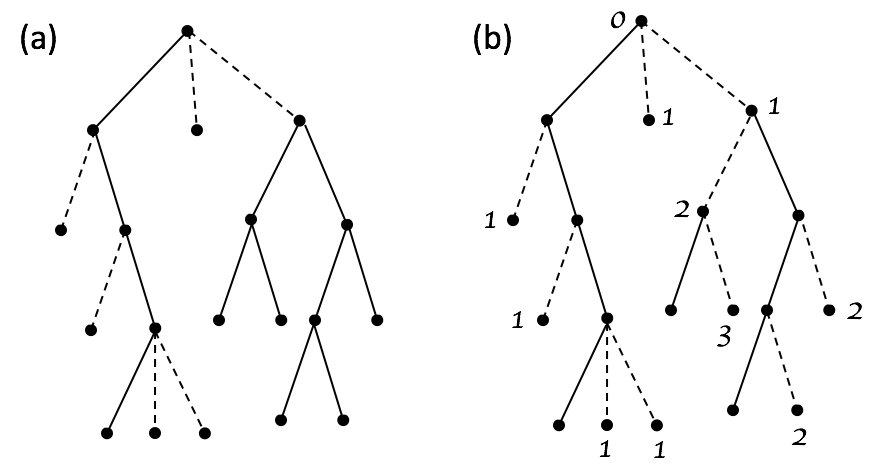
\includegraphics[scale=0.5]{centroid}
        \centering
        \caption{Demonstration of centroid path decomposition. Both (a) and (b) use the same tree. In (a), the tree has undergone a centroid path decomposition such that after the dashed edges are removed, leaving a centroid path and a set of side trees. In (b), the tree has undergone a complete centroid path decomposition, with the dashed edges being removed to leave only a set of paths.}
        \label{fig:centroid}
    \end{figure}

    \subsection{The \textit{delete} operation}
    \label{subsec:delete}

    As described in \cite{jansson2018algorithms}, the \textit{delete} operation deletes a cluster from a tree. To do so, we specify some internal node $u$ in a tree $T$, such that we wish to delete the cluster $\leafset^{T}(u)$. Then the \textit{delete} operation makes $parent(u)$ the parent of all nodes in $children(u)$ and removes $u$, along with any associated edges from $T$. This has the effect of removing only $\leafset(u)$ from $T$, without affecting any other cluster. For example, in Figure~\ref{fig:freqdiff}, if we perform a delete operation on $T_2$, on the node associated with the cluster $\{b, c\}$, the resulting tree is identical to $T_{FD}$.

    \subsection{Characterising incompatibility}

    We restate Lemma 6 of \cite{jansson2018algorithms} here since it is crucial in the development of an algorithm discussed below:
    \newline

    \begin{incompatibility}
        \label{lem:incompatibility}

        Given a tree $T$ and a cluster $C \subseteq \leafset(T)$, let $l_C = lca^T(C)$. Then for any $u \in V(T)$, $C \not\compatible \leafset(u)$ iff $u$ lies on the path between $l_C$ and some $x \in C$ and $\leafset(u) \not\subseteq C$.
    \end{incompatibility}

    \subsection{The \texttt{Merge\_Trees} algorithm}
    \label{subsec:mergetrees}

    We restate the following lemma outlining the \texttt{Merge\_Trees} operation from \cite{jansson2016improved}:
    \newline

    \begin{mergetrees}
        \label{lem:mergetrees}

        Given trees $T_1$ and $T_2$ where $\leafset^{T_1} = \leafset^{T_2} = L$ and $T_1 \compatible T_2$, \texttt{Merge\_Trees}$(T_1, T_2) = T$, where $\leafset^T = L$ and $\mathcal{C}(T) = \mathcal{C}(T_1) \cup \mathcal{C}(T_2)$. This algorithm runs in $O(|L|)$ time.
    \end{mergetrees}

    \begin{figure}[h]
        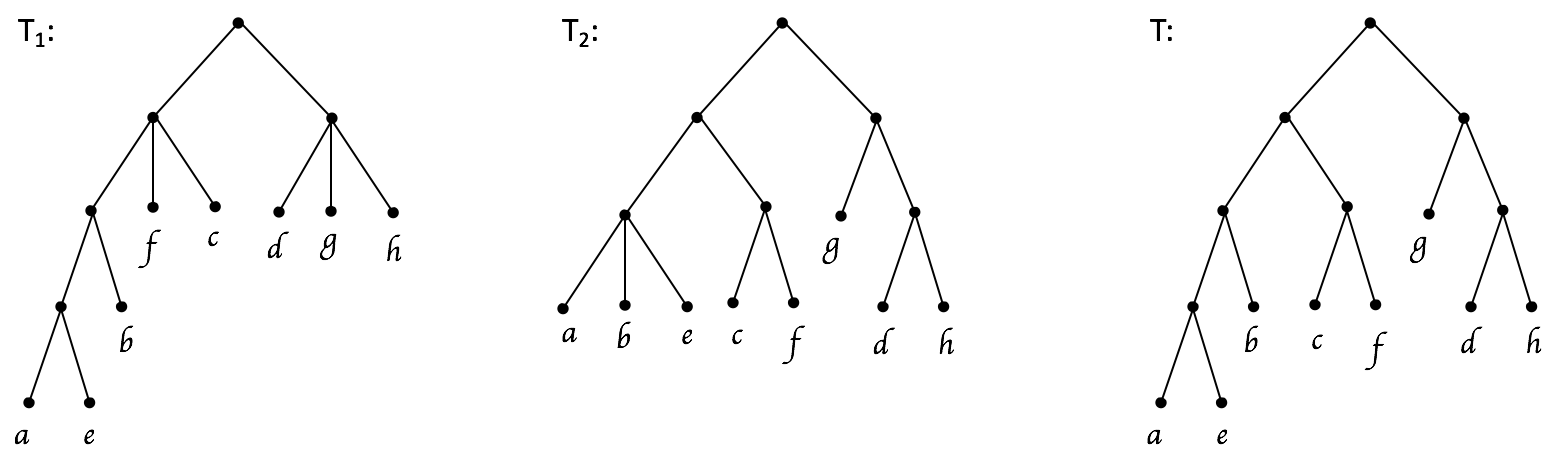
\includegraphics[scale=0.5]{mergetrees}
        \centering
        \caption{$T_1 \compatible T_2$. $T =$ \texttt{Merge\_Trees}$(T_1, T_2)$. $\mathcal{C}(T) = \mathcal{C}(T_1) \cup \mathcal{C}(T_2)$.}
        \label{fig:mergetrees}
    \end{figure}

    Figure~\ref{fig:mergetrees} gives an example for the \texttt{Merge\_Trees} algorithm. Here, $T_1 \compatible T_2$ and $T =$ \texttt{Merge\_Trees}$(T_1, T_2)$. Observe that,
    \begin{align*}
        \mathcal{C}(T_1) &= \{\{a, e\}, \{a, b, e\}, \{a, b, c, e, f\}, \{d, g, h\}\}\\
        \mathcal{C}(T_2) &= \{\{a, b, e\}, \{c, f\}, \{a, b, c, e, f\}, \{d, h\}, \{d, g, h\}\}\\
        \mathcal{C}(T) &= \{\{a, e\}, \{a, b, e\}, \{c, f\}, \{a, b, c, e, f\}, \{d, h\}, \{d, g, h\}\}\\
        &= \mathcal{C}(T_1) \cup \mathcal{C}(T_2).
    \end{align*}

    \subsection{The \texttt{Frequency\_Difference} algorithm}

    The algorithm \texttt{Frequency\_Difference} \cite{jansson2018algorithms} computes the FDCT of a set of trees $\mathcal{S}$. It runs in two parts. First, for any tree $T \in \mathcal{S}$ and any node $u \in V(T)$, it computes $\weight(u)$ in the \textit{weighting} step. In the second part, it utilises \texttt{Filter\_Clusters} (defined below) and \texttt{Merge\_Trees} (from Subsection~\ref{subsec:mergetrees}) to compute the FDCT.

    As in \cite{jansson2018algorithms}, the subprocedure \texttt{Filter\_Clusters}, is defined to take as input trees $\TA$ and $\TB$, with $\leafset^{\TA} = \leafset^{\TB} = L$ and the values of $\weight(u)$ for all $u \in V(\TA) \cup V(\TB)$. It returns a tree $T$ which contains all clusters $C$ in $\TA$ for which $\weight(C) > $ weights of all clusters in $\TB$ that are incompatible with $C$. Formally, \texttt{Filter\_Clusters}$(\TA, \TB) = T$ where $\mathcal{C}(T) = \{C : C \in \mathcal{C}(\TA) \text{ and } \weight(C) > max(\{\weight(C_1) : C_1 \in \mathcal{C}(\TB) \text{ and } C_1 \not\compatible C\})\}$ and $\leafset^T = L$. For example, referring to Figure~\ref{fig:freqdiff}, \texttt{Filter\_Clusters}$(T_2, T_1) = T_{FD}$. Notice that there are three non-trivial clusters in $T_2$: $\{a, b, c\}, \{b, c\}$ and $\{d, e\}$. All of these have weight $2$. Now the only cluster in $T_1$ incompatible with $\{a, b, c\}$ is $\{c, d, e\}$, but this only has weight $1$ and so $\{a, b, c\}$ is kept. The cluster $\{d, e\}$ is compatible with $T_1$ so it is also kept. However, $\{b, c\}$ is incompatible with $\{a, b\}$ and they both have weight $2$, hence $\{b, c\} \not\in \mathcal{C}($\texttt{Filter\_Clusters}$(T_2, T_1))$.

    Theorem 3 of \cite{jansson2018algorithms} gives the following corollary:
    \newline

    \begin{freqdiffruntimecomponents}
        \label{cor:freqdiffruntimecomponents}

        The total runtime of \texttt{Frequency\_Difference} is given by $O(g(n, k) + k \cdot f(n))$ where $g(n, k)$ is the time taken by the weighting step and $f(n)$ is the runtime of \texttt{Filter\_Clusters}.
    \end{freqdiffruntimecomponents}

    Jansson et al. \cite{jansson2018algorithms} gave a $min(\{O(kn^2), O(k^2n)\})$ solution to the weighting step and an $O(n\,log^2n)$ solution to \texttt{Filter\_Clusters}, giving an overall runtime of $min(\{O(kn^2), O(kn(k + log^2n))\})$. Gawrychowski et al. \cite{gawrychowski2017faster} improved the runtime of the weighting step to $O(kn\,log^2n)$, thus reducing the overall runtime to $O(kn\,log^2n)$.

    \section{$childD$ queries}
    \label{sec:cfd}

    Given a tree $T$ and nodes $v, w \in V(T)$ such that $w$ is a proper ancestor of $v$, define $childD(v, w)$ as the child of $w$ that is an ancestor of $v$. We construct a data structure that allows us to answer this query in constant time, given $O(n\,log\,n)$ preprocessing time, where $n = |V(T)|$.

    Reorder $T$ such that the heaviest child of each node is its leftmost child. Then the leaves of $T$ are indexed in left to right order, such that every leaf $x \in \leafset^T$ is assigned a value $index(x)$. Then for every node $u \in V(T)$, the indices of the leaves in $T[u]$ form a consecutive range. For each internal node $u \in V(T)$, define its side children to be the set $children(u) - \{\text{heaviest child of }u\}$ and its side trees to be the subtrees of $T$ rooted at its side children. Let $x$ and $y$ be the leaves in the side trees of $u$ with the smallest and largest indices respectively. We now build the array $cFL_u[0\, ...\, index(y) - index(x)]$ which maps each leaf $z$ in the side trees of $u$ to the child of $u$ that is an ancestor of $z$. Thus, for every leaf $z$ in $T[v]$ for some $v \in$ side children of $u$, let $cFL_u[index(z) - index(x)] = v$.
    \newline

    \begin{cfddatastructure}
        \label{lem:cfddatastructure}

        Given a tree $T$ where $n = |V(T)|$, the $cFL$ data structure defined above can be constructed in $O(n\,log\,n)$ time.

        \begin{proof}
            Rearranging $T$ and indexing the leaves can be done in two $O(n)$ passes. By the standard argument of centroid-path decomposition, we argue that any leaf is in the side trees of $O(log\,n)$ nodes, hence the total size of the $cFL$ arrays is $O(n\,log\,n)$. It is easy to see that these arrays can thus be constructed in $O(n\,log\,n)$ time.
        \end{proof}
    \end{cfddatastructure}

    \medskip
    \begin{cfdquery}
        \label{lem:cfdquery}

        Given a tree $T$, an $lca$ data structure on $T$, the $cFL$ data structure on $T$ and nodes $v, w \in V(T)$, the query $childD(v, w)$ can be answered in constant time.

        \begin{proof}
            The query is divided into two parts. First, we check if $v$ is a descendant of the heaviest child of $w$. If so, we are done. If not, we need to determine which child of $w$ is an ancestor of $v$.

            To answer the first part, we can see that, given nodes $r, s \in V(T)$, $s$ is an ancestor of $r$ iff $lca(r, s) = s$. Thus we can check if $v$ is a descendant of the heaviest child of $w$ in $O(1)$ time since by Lemma~\ref{lem:lca}, the $lca$ data structure allows queries in constant time.

            For the second part, we simply retrieve the entry corresponding to any leaf in $\leafset(v)$ from $cFL_w$, again easily done in constant time.
        \end{proof}
    \end{cfdquery}

    \section{RMQ structure on trees}
    \label{sec:rmqtree}

    Here, we generalise the linear RMQ data structure to trees. Given a tree $T$ and $\weight(u)$ for each $u \in V(T)$, for any nodes $v, w \in V(T)$ such that $w$ is an ancestor of $v$, let $rmqTree^T[v, w] = max_{u \in path^T[v, w]}\weight(u)$, where $path^T[v, w]$ is the set of all nodes on the path from $v$ to $w$, including both $v$ and $w$. Note that the square brackets are used to indicate inclusion of the two endpoints. We build a data structure for answering $rmqTree^T[v, w]$ queries in constant time, given $O(n\,log\,n)$ preprocessing time, where $n = |V(T)|$.

    The data structure outlined here builds on the one presented in Lemma 8 of \cite{jansson2018algorithms}, while providing some further details of the implementation. Firstly, for each centroid path $P_i \in \mathcal{P}(T)$, the weights along $P_i$ are stored in a linear RMQ structure (as described in Lemma~\ref{lem:linearrmq}). Then for each leaf $x \in \leafset^T$, the path from $x$ to the root of $T$ can be seen as a concatenation of subpaths of the aforementioned centroid paths. An example of this can be seen in Figure~\ref{fig:rmq}. This figure shows part of a tree. The diagonal lines from right to left are centroid paths in the tree (elements of $\mathcal{P}(T)$). The dashed edges indicate that the child is not the heaviest child of its parent, hence starting a new centroid path. As can be seen, the path from the leaf $x$ to the root consists of subpaths of many centroid paths. We denote these subpaths by $Q_1, Q_2, ..., Q_f$, where $Q_1$ contains $root(T)$ and $Q_f$ contains $x$. For each $x$, we build the array $W_x[1 ... f]$, where $W_x[i] = max_{u \in Q_i}\weight(u)$ and store this array in a linear RMQ structure.

    \begin{figure}[h]
        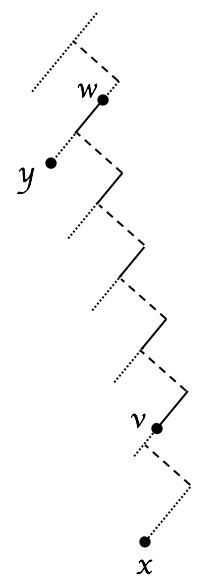
\includegraphics[scale=0.5]{rmq}
        \centering
        \caption{Demonstration of an $rmqTree[v, w]$ query. The diagonal lines from right to left are centroid paths of the tree. The parts in bold lie on the path between $v$ and $w$, while those that are dotted do not. Dashed lines connect the root of a centroid path to its parent. $y$ is the leaf at the bottom of the centroid path to which $w$ belongs. $x$ is some leaf in the subtree rooted at $v$. {\color{red} Has this been explained too many times?}}
        \label{fig:rmq}
    \end{figure}

    We also compute the depth of each node as the distance from the root of $T$. Further, the concept of depth is generalised to the centroid paths, where for any centroid path $P_i \in \mathcal{P}(T)$, $depth(P_i) = 1\, +$ depth of centroid path containing the parent of the root of $P_i$. Intuitively, if we build a tree from only the roots of the centroid paths while maintaining the same relative structure, then the depth of a centroid path would simply be the depth of its root in this new tree.
    \newline

    \begin{rmqdatastructure}
        \label{lem:rmqdatastructure}

        Given a tree $T$ and $\weight(u)$ for each $u \in V(T)$, the $rmqTree$ data structure can be built in $O(n\,log\,n)$ time.

        \begin{proof}
            The decomposition step, along with computation of depths for nodes and for centroid paths can be done in $O(n)$ time. Storing the centroid paths in linear RMQ structures takes $O(n)$ time, by Lemma~\ref{lem:linearrmq} and since the total size of the centroid paths is $O(n)$. By the standard argument of centroid-path decomposition, it can be seen that for each leaf $x$, the number of centroid subpaths on the path from the leaf to the root of $T$ is $O(log\,n)$. Hence it takes $O(log\,n)$ time to build the linear RMQ structure for these subpaths. Since there are $n$ leaves, the total time taken to construct the linear RMQ structures for all leaves is $O(n\,log\,n)$.
        \end{proof}
    \end{rmqdatastructure}

    \medskip
    \begin{rmqquery}
        \label{lem:rmqquery}

        Given a tree $T$, an $lca$ data structure on $T$, the $rmqTree$ data structure on $T$, and nodes $v, w \in V(T)$ such that $w$ is an ancestor of $v$, the query $rmqTree[v, w]$ can be answered in constant time.

        \begin{proof}
            We use the complete centroid path decomposition done when producing the $rmqTree$ data structure. The path from $v$ to $w$ is partitioned into a concatenation of subpaths of these centroid paths, denoted by $Q_1, Q_2, ..., Q_g$. This is illustrated in Figure~\ref{fig:rmq}. The diagonal lines from right to left are some of the centroid paths the tree has been decomposed into. The dashed edges indicate that the child is not the heaviest child of its parent, such that the child is the root of a new centroid path. The bold lines are the subpaths of centroid paths that lie on the path from $v$ to $w$. $Q_1$ is the bold centroid subpath starting from $v$ and continuing upwards till the root of that path. Similarly, $Q_g$ is the bold centroid subpath starting at $w$ and continuing downwards until the path splits from that centroid path. $Q_2$ to $Q_{g - 1}$ are the bold centroid subpaths between $Q_1$ and $Q_g$. The significance of the leaves $x$ and $y$ is explained below.

            Take any $x \in \leafset(v)$. Then $Q_2, ..., Q_{g - 1}$ are contained fully in the centroid subpaths on the path from $x$ to the root of $T$. $Q_1$ must be a subpath that starts at $v$ in some centroid path $\in \mathcal{P}(T)$ and ends at the root of that centroid path. $Q_g$ is a subpath that starts at some node in some centroid path $\in \mathcal{P}(T)$ and ends at $w$, within the same path. We address each of these three divisions separately.

            To find the maximum weight within $Q_1$, we obtain the depth of $v$ within $Q_1$ by subtracting the depth of the root of $Q_1$ from the depth of $v$. Then the maximum weight can be retrieved by querying the linear RMQ structure for this centroid path, from the root to $v$ (recall that the depths and linear RMQ structures were obtained while constructing the $rmqTree$ data structure). Querying the linear RMQ structure costs constant time, as set out in Lemma~\ref{lem:linearrmq}.

            To find the maximum weight for the subpaths $Q_2, ..., Q_{g - 1}$, we obtain the indices of $Q_2$ and $Q_{g-1}$ in $W_x$ as $depth(Q_1) + 1$ and $depth(Q_g) - 1$ respectively. The maximum weight can then be found by querying $W_x$.

            Finally, we need to find the maximum weight within $Q_g$. Observe that the key here is finding which node is at the end of $Q_g$. Let $P_i \in \mathcal{P}(T)$ be the centroid path of which $Q_g$ is a subpath. Then the previous question is equivalent to finding which node in $P_i$ has $v$ in one of its side trees. Let $y$ be the leaf at the bottom of $P_i$. Then the desired node is simply $lca(y, v)$, querying for which takes $O(1)$ time as given by Lemma~\ref{lem:lca}. The maximum weight within $Q_g$ can now be easily found in constant time by querying the linear RMQ structure for $P_i$, from $w$ to $lca(y, v)$.

            As of these three values can be obtained in constant time, the query as a whole takes $O(1)$ time.
        \end{proof}
    \end{rmqquery}

    \section{Weighting}
    \label{sec:weighting}

    Given the set of trees $\mathcal{S} = \{T_1, T_2, ..., T_k\}$, where $\leafset(T_1) = \leafset(T_2) = ... = \leafset(T_k) = L$ and $n = |L|$, the weighting step computes $\weight(u)$ for every node $u \in \bigcup_{T \in \mathcal{S}}V(T)$. Recall that $\weight(u)$ gives the frequency of $\leafset(u)$ in $\mathcal{S}$. We divide this work (as in \cite{gawrychowski2017faster}) into the labelling and counting steps. The labelling step assigns a label to each node $u \in T, T \in \mathcal{S}$, denoted by $id(u)$, such that $id(u) \in [1 ... 2kn]$ and for any node $u' \in T', T' \in \mathcal{S}$, $id(u) = id(u')$ iff $\leafset^T(u) = \leafset^{T'}(u')$. That is, two nodes have the same label iff they are associated with the same cluster. The counting step sorts these labels, allowing us to count how many nodes exist with each label, giving us the frequencies (or the weights) of the nodes.

    Recall that the approach in \cite{gawrychowski2017faster} costs $O(kn\,log^2n)$ time. We develop a way to achieve $O(kn\,log\,n)$ time.

    The idea here will be to divide $L$ into two equal sized halves, $L'$ and $L''$. Then, we wish to build the sets $\{\leafset^T(u) \cap L' : T \in \mathcal{S}, u \in V(T)\}$ and $\{\leafset^T(u) \cap L'' : T \in \mathcal{S}, u \in V(T)\}$. If each of these sets could be labelled such that each cluster within them has a unique label, then for any tree $T \in \mathcal{S}$, for any node $u \in V(T)$, $\leafset^T(u)$ is uniquely identified by the pair $(id(\leafset^T(u) \cap L'), id(\leafset^T(u) \cap L''))$. To be able to achieve this, we introduce the definitions below.

    First, for any tree $T$ and any cluster $C \subseteq \leafset(T)$, define $T|C$, read as ``$T$ restricted to $C$'', as the tree $T'$ with $V(T') = \{lca^T(u, v) : u, v \in C\}$ which obeys $lca^T(C') = lca^{T'}(C')$ for all $C' \subseteq C$. Intuitively, $T'$ has the leaf set $C$ and consists of all nodes in $T$ that are $lca$'s of the leaves in $C$, with these nodes connected such that they have the same ancestor/descendant relationships as they had in $T$. Figure~\ref{fig:labelclusters} demonstrates this process; the tree $T_1|L'$ is $T_1$ restricted to the cluster $\{a, b, c, d\}$. Notice that nodes which are not $lca$'s of these leaves are removed, but the structure of the tree in relation to these leaves remains the same.

    Further, for every cluster $C \subseteq L$, and every node $u$ in $T$, define the node $assoc^C(u) = lca^T(C \cap \leafset^T(u))$. Notice that if $C \cap \leafset^T(u) \neq \emptyset$, $assoc^C(u) \in V(T|C)$ since it is the $lca$ of some non-empty subset of $C$. However, if $C \cap \leafset^T(u) = \emptyset$, then for convenience let $assoc^{C}(u) = \Phi$, where $\Phi$ is a special node with $id(\Phi) = 0$ and $\leafset(\Phi) = \emptyset$. We refer to Figure~\ref{fig:labelclusters} to show examples of this concept. Let $u$ and $v$ be the nodes in $T_1$ labelled $(5, 1)$ and $(5, 0)$ respectively. Then $assoc^{\{a, b, c, d\}}(u) = v$, since $v = lca^{T_1}(\{a, b, c, d\} \cap \leafset^{T_1}(u)) = lca^{T_1}(\{a, b\})$. $assoc^{\{e, f, g, h\}}(v) = \Phi$, since $\leafset^{T_1}(v) \cap \{e, f, g, h\} = \emptyset$.

    Using these observations, we can expand on the previous description of the algorithm. We divide $L$ into $L'$ and $L''$, then we construct and recursively label the sets $\{T|L' : T \in \mathcal{S}\}$ and $\{T|L'' : T \in \mathcal{S}\}$. Then for any tree $T \in \mathcal{S}$, for any node $u \in V(T)$, $\leafset^T(u)$ can be represented by the pair $(id(assoc^{L'}(u)), id(assoc^{L''}(u)))$. Once we obtain these pairs, we sort them and assign a rank to each unique pair; $id(u)$ is then the rank of the pair $(id(assoc^{L'}(u)), id(assoc^{L''}(u)))$. The resulting algorithm \texttt{Label\_Clusters} is laid out below.

    \begin{algorithm}
        \caption{Label\_Clusters}
        \label{alg:labelclusters}

        \begin{algorithmic}[1]
            \Input A set $\mathcal{S}$ of trees $\{T_1, T_2, ..., T_k\}$ where $\leafset(T_1) = \leafset(T_2) = ... = \leafset(T_k) = L$

            \Output Associate a label $id(u) \in [1 ... 2k |L|]$ with every node $u$ in the trees in $\mathcal{S}$ such that for any two nodes $v, w$ in some trees in $\mathcal{S}$, $id(v) = id(w)$ iff $\leafset(v) = \leafset(w)$.

            \State Partition $L$ into $L'$ and $L''$ such that $|L'| = |L''|$.

            \State For all $i \in [1 ... k]$, let $T'_i = T_i|L'$ and $T''_i = T_i|L''$.

            \State \texttt{Label\_Clusters}$(\{T'_1, T'_2, ..., T'_k\})$.

            \State \texttt{Label\_Clusters}$(\{T''_1, T''_2, ..., T''_k\})$.

            \State For every tree $T \in \mathcal{S}$, for every node $u \in T$, represent $u$ by the pair $(id(assoc^{L'}(u)), id(assoc^{L''}(u)))$.

            \State Radix sort all pairs obtained and remove duplicates. Assign a rank to each unique pair.

            \State For every tree $T \in \mathcal{S}$, for every node $u \in T$, set $id(u) = $ rank of the pair $(id(assoc^{L'}(u)), id(assoc^{L''}(u)))$.
        \end{algorithmic}
    \end{algorithm}

    One iteration of this process is illustrated in Figure~\ref{fig:labelclusters}. Here $L' = \{a, b, c, d\}$ and $L'' = \{e, f, g, h\}$. It is assumed that the algorithm has correctly labelled the clusters for each of the restricted trees, and these labels are assigned as shown in Figure~\ref{fig:labelclusters}(b). Figure~\ref{fig:labelclusters}(a) then shows the pair associated with each internal node of $T_1$ and $T_2$. For example, the cluster $\{a, b, e\}$ in $T_1$ is labelled by $5$ from $\{a, b\}$ in $T_1|L'$ and $1$ from $\{e\}$ in $T_1|L''$. Similarly, the cluster $\{a, b\}$ in $T_1$ is labelled by $5$ from $\{a, b\}$ in $T_1|L'$ and $0$ from $\Phi$ since $\{a, b\} \cap \{e, f, g, h\} = \emptyset$.

    \begin{figure}[h]
        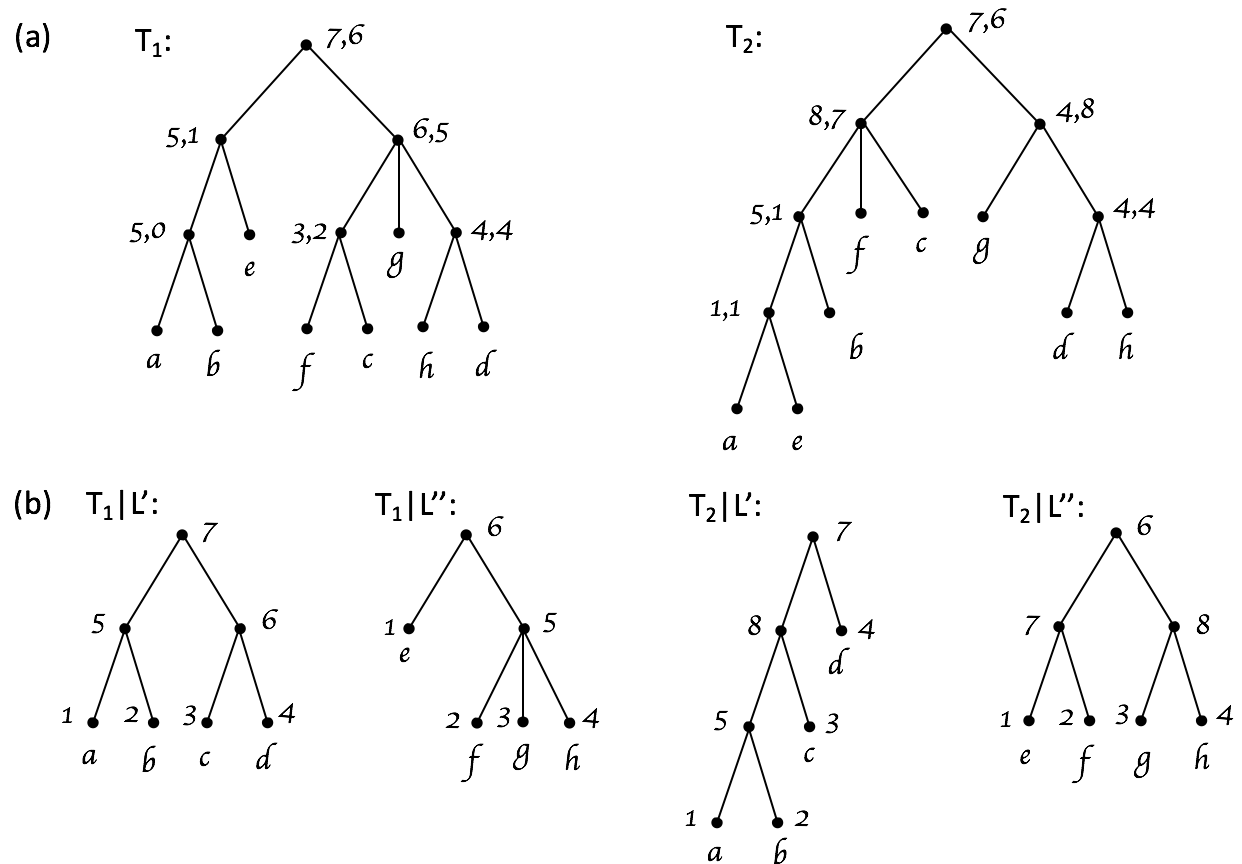
\includegraphics[scale=0.5]{labelclusters}
        \centering
        \caption{Demonstration of \texttt{Label\_Clusters}$(T_1, T_2)$. $L' = \{a, b, c, d\}$ and $L'' = \{e, f, g, h\}$. (b) shows the trees $T_1|L', T_1|L'', T_2|L'$ and $T_2|L''$, where these have been recursively labelled. The labels are shown beside each of the nodes. (a) shows the trees $T_1$ and $T_2$ where the pair that represents each node (except the leaves) is shown beside it.}
        \label{fig:labelclusters}
    \end{figure}

    {\color{red} I removed the shallowest descendant part completely, under the assumption that the process by which $assoc^C(u)$ is obtained is not hard to come up with. Is this reasonable, or should I prove something like $assoc^C(u) = $ shallowest descendant of $u$ in $T|C$?}

    The following Lemma proves the correctness of the given algorithm:

    \bigskip
    \begin{labelclusterscorrectness}
        \label{lem:labelclusterscorrectness}

        After running \texttt{Label\_Clusters}$(\mathcal{S})$, for any trees $T_i, T_j \in \mathcal{S}$, for any nodes $u \in V(T_i), v \in V(T_j)$, $id(u) = id(v)$ iff $\leafset^{T_i}(u) = \leafset^{T_j}(v)$.

        \begin{proof}
            $id(u) = id(v)$ iff $id(assoc^{L'}(u)) = id(assoc^{L'}(v))$ and $id(assoc^{L''}(u)) = id(assoc^{L''}(v))$. Inductively, $id(assoc^{L'}(u)) = id(assoc^{L'}(v))$ iff $\leafset^{T_i|L'}(assoc^{L'}(u)) = \leafset^{T_j|L'}(assoc^{L'}(v))$. By definition of the $assoc$ relation, $\leafset^{T_i}(u)\, \cap\, L' = \leafset^{T_j}(v)\, \cap\, L'$. Symmetrically, $id(assoc^{L''}(u)) = id(assoc^{L''}(v))$ iff $\leafset^{T_i}(u)\, \cap\, L'' = \leafset^{T_j}(v)\, \cap\, L''$. Since $L'$ and $L''$ partition $L$, both parts are true iff $\leafset^{T_i}(u) = \leafset^{T_j}(v)$.
        \end{proof}
    \end{labelclusterscorrectness}

    \medskip
    \begin{labelclustersidbounds}
        \label{lem:labelclustersidbounds}

        After running \texttt{Label\_Clusters}$(\mathcal{S})$, for any node $u \in V(T), T \in \mathcal{S}$, $id(u) \in [1 ... 2k |L|]$.

        \begin{proof}
            It is easily seen that $|V(T)| < 2|L|$. Thus the total number of pairs is less than $2k|L|$. This also places an upper bound on the number of ids. Notice that $u$ cannot be labelled with $0$ since that is reserved for the special node.
        \end{proof}
    \end{labelclustersidbounds}

    \medskip
    \begin{labelclustersruntime}
        \label{lem:labelclustersruntime}

        The algorithm \texttt{Label\_Clusters}$(\mathcal{S})$ runs in $O(kn\,log\,n)$ time.

        \begin{proof}
            Let $T(m)$ be the runtime of \texttt{Label\_Clusters}$(\mathcal{T})$, where $m =$ size of leaf set of each tree in $\mathcal{T}$. By Lemma 5.2 of \cite{farach1995fast}, construction of $T'_i$ and $T''_i$ takes $O(m)$ time for each $T_i \in \mathcal{T}$, taking total $O(km)$ time over all the trees. Computing $assoc^{L'}(u)$ and $assoc^{L''}(u)$ for each node $u$ in some tree $T_i \in \mathcal{T}$ can be done by a bottom up traversal of $T_i$ along with $T'_i$ and $T''_i$, taking $O(km)$ time total. Also observe that the number of pairs obtained is $O(km)$. Further, each of the values in the pair is in the range [0, km]. Thus radix sorting these pairs and assigning labels back to the nodes takes $O(km)$ time. So $T(m) = 2T(m/2) + O(km)$, giving $T(n) = kn\,log\,n$.
        \end{proof}
    \end{labelclustersruntime}

    \medskip
    \begin{weightingruntime}
        \label{lem:weightingruntime}

        The weighting step can be completed in $O(kn\,log\,n)$ time.

        \begin{proof}
            As shown in Lemma~\ref{lem:labelclustersruntime}, assigning labels to each node takes $O(kn\,log\,n)$ time. Next, we sort the labels by counting sort. Since each label is in the range $[1 ... 2kn]$ and there are $O(kn)$ labels, this takes $O(kn)$ time. The frequencies, or weights, can then be computed in $O(kn)$ time.
        \end{proof}
    \end{weightingruntime}

    \section{\texttt{Filter\_Clusters}}
    \label{sec:filterclusters}

    Given the trees $\TA$ and $\TB$ where $\leafset^{\TA} = \leafset^{\TB} = L$ and $n = |L|$, the algorithm \texttt{Filter\_Clusters}$(\TA, \TB)$ returns a tree $T$, where $\mathcal{C}(T) = \{C : C \in \mathcal{C}(\TA) \text{ and } \weight(C) > max(\{\weight(C_1) : C_1 \in \mathcal{C}(\TB) \text{ and } C_1 \not\compatible C\})\}$ and $\leafset(T) = L$. Recall that the previous best known solution, as in \cite{jansson2018algorithms}, costs $O(kn\,log^2n)$ time; we present an $O(kn\,log\,n)$ solution.

    The key here is finding, for any node $u \in V(\TA)$, the set of nodes in $\TB$ that are incompatible with $u$, so that we can find the maximum weight of these. Then it is easy to figure out whether $u$ should be in $T$ or not.

    % In Subsection~\ref{subsec:rootsofsubtrees} we describe an insight into the structure of trees that later leads to an improvement in the time taken to find this set of incompatible nodes. Subsection~\ref{subsec:incompatibilityrecursive} uses this idea to give a stricter definition of incompatibility, and finally Subsection~\ref{subsec:filterclustersalgorithm} uses this definition to present our solution for \texttt{Filter\_Clusters}.

    \subsection{Minimum Cover}
    \label{subsec:minimumcover}

    This section presents an insight into the structure of the trees under consideration, later shown to be the key to decreasing the runtime of the algorithm.

    Given a tree $T$ and a cluster $C \subseteq L$, define a set $S \subseteq V(T)$ to be a cover of $C$ in $T$ if $\bigcup_{u \in S} \leafset^{T}(u) = C$. Then we define the minimum cover of $C$ in $T$, denoted as $minCover^{T}(C)$, to be the smallest set $S$ such that $S$ is a cover of $C$. Note that this set is well defined for each cluster.

    As will be shown in Subsection~\ref{subsec:incompatibilityrecursive}, the minimum cover of a cluster $C$ is crucial in finding the set of nodes incompatible with $C$. Thus we would like to build a means of obtaining the minimum cover of a cluster $C$. Observe that for any leaf $x \in \leafset^T$, $minCover^T(\{x\}) = \{x\}$. We now build a recursive definition for $minCover$.

    \begin{mincoverrecursive}
        \label{lem:mincoverrecursive}

        Given a tree $T$, a cluster $C \subseteq L$ and a node $u \in V(T)$ such that $\leafset^{T}(u) \cap C = \emptyset$, let $S = minCover^{T}(C)$. Then $minCover^{T}(C \cup \leafset^{T}(u)) = \begin{cases}
            a \\ b \\ c
        \end{cases}$
    \end{mincoverrecursive}

    Given a tree $T$, cluster $C \subseteq L$, for any node $r \in V(T)$, define $r$ to be the root of a \textit{maximal subtree compatible with $C$} if (1) $\leafset^T(r) \subseteq C$ and (2) $\leafset^T(r') \not\subseteq(C)$ for all proper ancestors $r'$ of $r$. The set $RST^{T}(C)$ is composed of all nodes $r \in V(T)$ that are roots of maximal subtrees compatible with $C$. Extending this, given any node $u$, we denote $RST^{T}(\leafset(u))$ as $RST^{T}(u)$. For example, in the tree in Figure~\ref{fig:rootsofsubtrees}, the circled nodes are roots of maximal subtrees compatible with $C = \{a, b, c, f, g, h\}$, i.e. $RST^{T}(C)$.

    As will be shown in Subsection~\ref{subsec:incompatibilityrecursive}, the roots of subtrees are crucial in finding the set of incompatible nodes. Thus, for every node $u \in V(\TA)$, we would like to compute $RST^{\TB}(u)$. However, we will solve a related problem: for any internal node $p_i \in \pi(\TA)$, we will use $RST^{\TB}(p_{i-1})$ and the set $boundary^{\TB}(p_i) = \bigcup_{c \in children(p_i)\, \backslash\, p_{i-1}} RST^{\TB}(c)$ to compute $RST^{\TB}(p_i)$. Note that $boundary^{\TB}(p_i)$ is the set of all roots of subtrees for the side trees associated with $p_i$.

    \begin{figure}[h]
        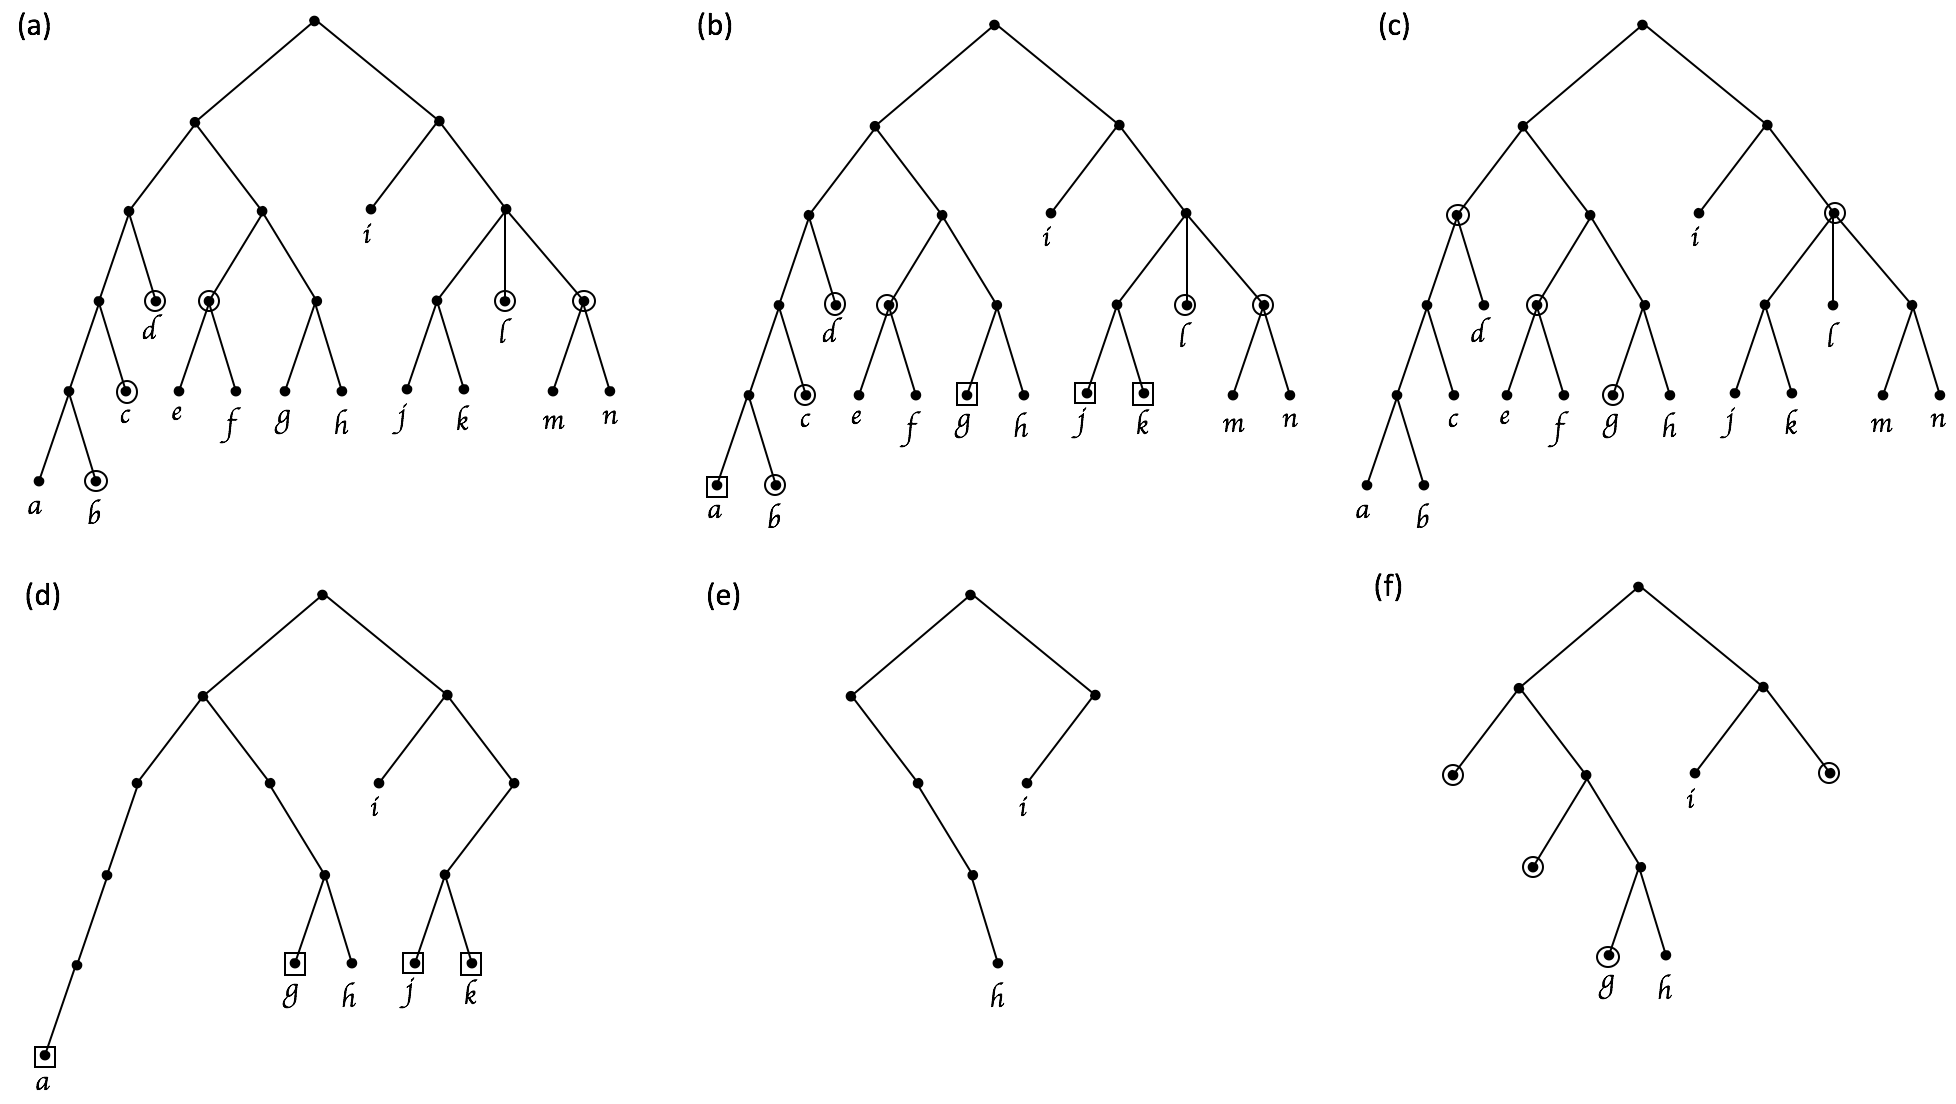
\includegraphics[scale=0.4]{rootsofsubtreesrecursive}
        \centering
        \caption{Demonstration of \texttt{Compute\_Roots\_Of\_Subtrees}. Here, $\leafset^{\TA}(p_{i-1}) = \{b, c, d, e, f, l, m, n\}$ and $\leafset^{\TA}(p_i) = \{a, b, c, d, e, f, g, j, k, l, m, n\}$. In (a), nodes belonging to $RST^{\TB}(p_{i-1})$ are marked with circles. The leafsets of the side trees associated with $p_i$ are $\{a, j\}$ and $\{g, k\}$. Thus (b) shows all nodes in $boundary^{\TB}(p_i)$ marked with squares, while nodes in $RST^{\TB}(p_{i-1})$ remain marked with circles. Finally, we see nodes in $RST^{\TB}(p_i)$ marked with circles in (c). The labels next to the nodes in (a) and (c) give the counter values at those nodes before and after \texttt{Compute\_Roots\_Of\_Subtrees} is used for $p_i$ respectively.}
        \label{fig:rootsofsubtreesrecursive}
    \end{figure}

    We illustrate with the example in Figure~\ref{fig:rootsofsubtreesrecursive}. For some non-leaf node $p_i \in \pi(\TA)$, we let $\leafset^{\TA}(p_{i-1}) = \{b, c, d, e, f, l, m, n\}$ and $\leafset^{\TA}(p_i) = \{a, b, c, d, e, f, g, j, k, l, m, n\}$. Figure~\ref{fig:rootsofsubtreesrecursive}(a) shows $\TB$ with all nodes in $RST^{\TB}(p_{i-1})$ marked with circles. Let the leafsets of the side trees associated with $p_i$ be $\{a, j\}$ and $\{g, k\}$. Figure~\ref{fig:rootsofsubtreesrecursive}(b) shows $\TB$ with all nodes in $boundary^{\TB}(p_i)$ marked with squares (the nodes from (a) remain marked with circles).

    Now Figure~\ref{fig:rootsofsubtreesrecursive}(c) shows $\TB$ with nodes in $RST^{\TB}(p_i)$ marked with circles. Thus the problem to be solved is going from the marked nodes in (b) to the marked nodes in (c). Observe that the only nodes that are new candidates for $RST^{\TB}(p_i)$ (as compared to $RST^{\TB}(p_{i-1})$) are ancestors of nodes in $boundary^{\TB}(p_i)$. Thus the idea here will be to initialise a set of candidate nodes with $RST^{\TB}(p_{i-1})$ and then iterate upwards from the nodes in $boundary^{\TB}(p_i)$, discovering nodes on the way that have leafsets which are subsets of $\leafset^{\TA}(p_i)$. In particular, if it turns out that for some node $v \in V(\TB)$, all the children of $v$ are in our set of candidates, then it must be true that for each node $c \in children(v)$, $\leafset^{\TB}(c) \subseteq \leafset^{\TA}(p_i)$, which implies that $\leafset^{\TB}(v) \subseteq \leafset^{\TA}(p_i)$. Thus at this point, we can add $v$ to our set of candidates and remove all children of $v$ from this set.

    Notice that to implement this process, we need a quick way of checking whether all the children of $v$ are in the set of candidates. We leave this detail as a black box for now, with the claim that it can be done in constant time. The actual method of doing so is provided in Lemma~\ref{lem:maintainingcounter}.

    Finally, it will be seen later that rather than simply computing $RST^{\TB}(p_i)$, it is desirable to compute three sets (in the following definitions, $u \in V(\TA)$ and $c \in children(u)$):

    \begin{align*}
        newRST^{\TB}(u, c) &= RST^{\TB}(u) - RST^{\TB}(c)\\[0.5em]
        removedRST^{\TB}(u, c) &= RST^{\TB}(c) - RST^{\TB}(u)\\[0.5em]
        oldRST^{\TB}(u, c) &= RST^{\TB}(u) \cap RST^{\TB}(c)
    \end{align*}

    In particular, we wish to find $newRST^{\TB}(p_i, p_{i-1})$, $removedRST^{\TB}(p_i, p_{i-1})$ and $oldRST^{\TB}(p_i, p_{i-1})$. We thus present the procedure \texttt{Compute\_Roots\_Of\_Subtrees} (Algorithm~\ref{alg:computerootsofsubtrees}) which, for some trees $\TA$ and $\TB$ where $\leafset^{\TA} \subseteq \leafset^{\TB}$ and some node $p_i \in \pi(\TA)$, takes as input $RST^{\TB}(p_{i-1})$, $boundary^{\TB}(p_i)$ and $\TB$. It returns the sets $newRST^{\TB}(p_i, p_{i-1})$, $removedRST^{\TB}(p_i, p_{i-1})$ and $oldRST^{\TB}(p_i, p_{i-1})$.

    \begin{algorithm}
        \caption{Compute\_Roots\_Of\_Subtrees}
        \label{alg:computerootsofsubtrees}

        \begin{algorithmic}[1]
            \Input For some trees $\TA$ and $\TB$, where $\leafset^{\TA} \subseteq \leafset^{\TB}$, and some internal node $p_i \in \pi(\TA)$, $RST^{\TB}(p_{i-1})$, $boundary^{\TB}(p_i)$ and $\TB$.

            \Output $newRST^{\TB}(p_i, p_{i-1})$, $removedRST^{\TB}(p_i, p_{i-1})$ and $oldRST^{\TB}(p_i, p_{i-1})$.

            \State $old := RST^{\TB}(p_{i-1})$

            \State $new, removed := \{\}$

            \ForAll{$v \in boundary$}
                \State $new := new \cup \{v\}$

                \State $v := parent(v)$

                \While{all children of $v$ are candidates}
                    \State $new := (new \cup \{v\}) - children(v)$

                    \State $removed := removed \cup (children(v) \cap old)$

                    \State $old := old - children(v)$

                    \State $v := parent(v)$
                \EndWhile
            \EndFor

            \State \Return $new, removed, old$
        \end{algorithmic}
    \end{algorithm}

    \bigskip
    \begin{computerootsofsubtreesruntime}
        \label{lem:computerootsofsubtreesruntime}

        For any trees $\TA$ and $\TB$ where $\leafset^{\TA} \subseteq \leafset^{\TB}$, for any internal node $p_i \in \pi(\TA)$, the algorithm \texttt{Compute\_Roots\_Of\_Subtrees}$(RST^{\TB}(p_{i-1}), boundary^{\TB}(p_i), \TB)$ runs in\\ % Overflows otherwise
        $O(|boundary^{\TB}(p_i)| + |removedRST^{\TB}(p_i, p_{i-1})|)$ time.

        \begin{proof}
            We implement each of the set of nodes using a linked list, while augmenting the nodes with a property that lets us know whether it belongs to the set or not. This allows us to perform operations like union, intersection and set difference in time proportional to the size of either of the sets.

            The outer loop is entered $O(|boundary^{\TB}(p_i)|)$ times.

            No node is added to $removed$ twice. This is because when a node $v$ is added to $removed$, $\leafset^{\TB}(parent(v)) \subseteq \leafset^{\TA}(p_i)$. Then $v$ can never be encountered again when iterating upwards any node in $boundary^{\TB}(p_i)$. Thus the total cost of the processing inside the inner loop is $O(|removedRST^{\TB}(p_i, p_{i-1})|)$.

            Notice that we reuse the list $(RST^{\TB}(p_{i-1})$ for $old$ to ensure that extra time is not spent copying this.

            Thus the total time taken is $O(|boundary^{\TB}(p_i)| + |removedRST^{\TB}(p_i, p_{i-1})|)$.
        \end{proof}
    \end{computerootsofsubtreesruntime}

    \begin{maintainingcounter}
        \label{lem:maintainingcounter}

        For any trees $\TA$ and $\TB$ where $\leafset^{\TA} \subseteq \leafset^{\TB}$, for any internal node $p_i \in \pi(\TA)$, when running the algorithm \texttt{Compute\_Roots\_Of\_Subtrees}$(RST^{\TB}(p_{i-1}), boundary^{\TB}(p_i), \TB)$, it is possible to check whether all the children of $v$ are in the set of candidates for any node $v \in V(\TB)$ in constant time.

        \begin{proof}
            We maintain a property $counter(v)$ for each node $v \in V(\TB)$. This property maintains the number of children of $v$ that are in either $new$ or $old$. Thus we can check whether they are all candidates by simply comparing $counter(v)$ with $|children(v)|$.

            To maintain this property correctly, when a node $v$ is added to $new$ during the procedure, $counter(parent(v))$ is incremented by one. Counters are never decremeneted because if some node $v$ is removed from the candidates, then $parent(v)$ is added to these candidates and since $parent(v)$ is never again encountered, there is no need to decrement $counter(parent(v))$.

            Notice that we require counters to be correct with respect to the nodes in $RST^{\TB}(p_{i-1})$. Thus we need some counter values to be set before \texttt{Compute\_Roots\_Of\_Subtrees} is called, and we will see this done later when the procedure is used as part of a larger algorithm.

            Observe that when the procedure terminates, the counter values are such that they are correct with respect to $RST^{\TB}(p_i)$, and thus these can be used for when calling the procedure on $p_{i+1}$.

            Figure~\ref{fig:rootsofsubtreesrecursive} demonstrates this process. Figure~\ref{fig:rootsofsubtreesrecursive}(a) shows the counter values before the procedure is called. Thus we see that, for example, the node labelled $2$ has two circled nodes as children. Then, we we iterate upwards from say the leaf $a$, we update the counter values and our candidate set until we end up with the situation in Figure~\ref{fig:rootsofsubtreesrecursive}(c) where the parent of the subtree with leafset $\{a, b, c, d\}$ has a counter value of $1$.
        \end{proof}
    \end{maintainingcounter}

    \subsection{Recursively determining incompatible nodes}
    \label{subsec:incompatibilityrecursive}

    Here we discuss how the concept of maximal compatible subtrees leads to a stricter definition of incompatibility and its implications for our algorithm.

    For any node $u \in V(\TA)$ and tree $\TB$, let the set $incompatible^{\TB}(u) = \{v : v \in V(\TB) \text{ and } \leafset^{\TB}(v) \not\compatible \leafset^{\TA}(u)\}$. Further, for any tree $T$ and nodes $v, w \in V(T)$ where $w$ is a proper ancestor of $v$, let $path^T(v, w)$ be the set of all nodes on the path from $v$ to $w$, excluding both these nodes. Note that $path^T(v, w) = path^T[parent^T(v), childD^T(v, w)]$.

    We now prove a stronger version of Lemma~\ref{lem:incompatibility} that takes the aforementioned maximal compatible subtrees into account to compute $incompatible^{\TB}(u)$ for any $u \in V(\TA)$.
    \newline

    \begin{incompatibilityrootsofsubtrees}
        \label{lem:incompatibilityrootsofsubtrees}

        Given trees $\TA, \TB$ and node $u \in V(\TA)$, $incompatible^{\TB}(u) = \bigcup_{r \in RST^{\TB}(u)} path^{\TB}(r, l_u)$, where $l_u = lca^{\TB}(\leafset^{\TA}(u))$.

        \begin{proof}
            $\longrightarrow$. For any $v \in V(\TB)$ such that $\leafset^{\TB}(v) \not\compatible \leafset^{\TA}(u)$, $v$ must be a proper descendant of $l_u$ by Lemma~\ref{lem:incompatibility}. Further, for some $x \in \leafset^{\TA}(u)$, $v$ is a proper ancestor of $x$ by Lemma~\ref{lem:incompatibility}. Then there must be some $r \in RST^{\TB}(u)$ such that $r$ is an ancestor of $x$. $v \not\in V(\TB[r])$, otherwise $\leafset^{\TB}(v) \subseteq \leafset^{\TA}(u)$. Thus $v$ is a proper ancestor of $r$ and $v \in path^{\TB}(r, l_u)$.

            $\longleftarrow$. Given some $v \in V(\TB)$ and $r \in RST^{\TB}(u)$ such that $v \in path^{\TB}(r, l_u)$, $\leafset^{\TA}(u) \not\subseteq \leafset^{\TB}(v)$, since $v$ is a proper descendant of $l_u$. Since $v$ is a proper ancestor of $r$, $\leafset^{\TB}(r) \subset \leafset^{\TB}(v)$, so $\leafset^{\TB}(v) \cap \leafset^{\TA}(u) \neq \emptyset$. Finally, $\leafset^{\TB}(v) \not\subseteq \leafset^{\TA}(u)$, otherwise $r \not\in RST^{\TB}(u)$. Thus $\leafset^{\TB}(v) \not\compatible \leafset^{\TA}(u)$.
        \end{proof}
    \end{incompatibilityrootsofsubtrees}

    This is illustrated in Figure~\ref{fig:rootsofsubtrees}. Here, any node in $RST^{\TB}(\{a, b, c, f, g, h\})$ is circled and any node that is incompatible with this cluster has a square around it. The node $l_u = lca^{\TB}(\{a, b, c, f, g, h\})$. As can be seen, all nodes on the path from roots of maximal subtrees to $l_u$ are incompatible with the given cluster.

    \begin{figure}[h]
        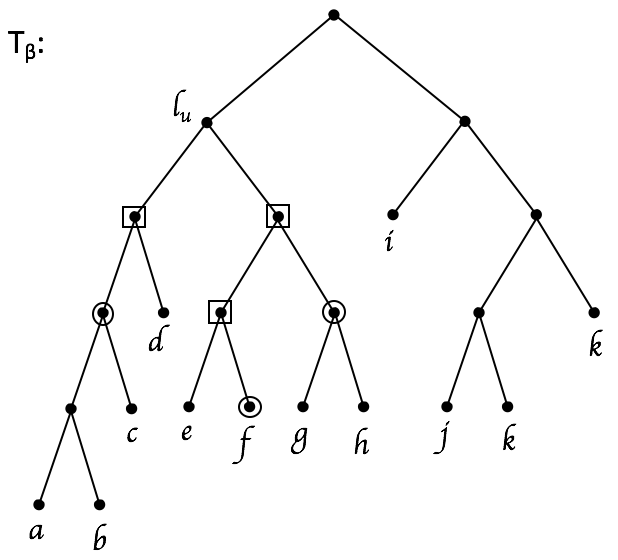
\includegraphics[scale=0.5]{rootsofsubtrees}
        \centering
        \caption{Illustration of Lemma~\ref{lem:incompatibilityrootsofsubtrees}. Let $C = \{a, b, c, f, g, h\}$. Then $l_u = lca^{\TB}(C)$. All circled nodes belong to $RST^{\TB}(C)$ and all nodes with a square around them belong to $incompatible^{\TB}(C)$.}
        \label{fig:rootsofsubtrees}
    \end{figure}

    We can now build, for any trees $\TA$ and $\TB$ and internal node $u \in V(\TA)$, a recursive definition of $incompatible^{\TB}(u)$, in terms of $incompatible^{\TB}(c_1)$, where $c_1 \in children(u)$.

    \begin{figure}[h]
        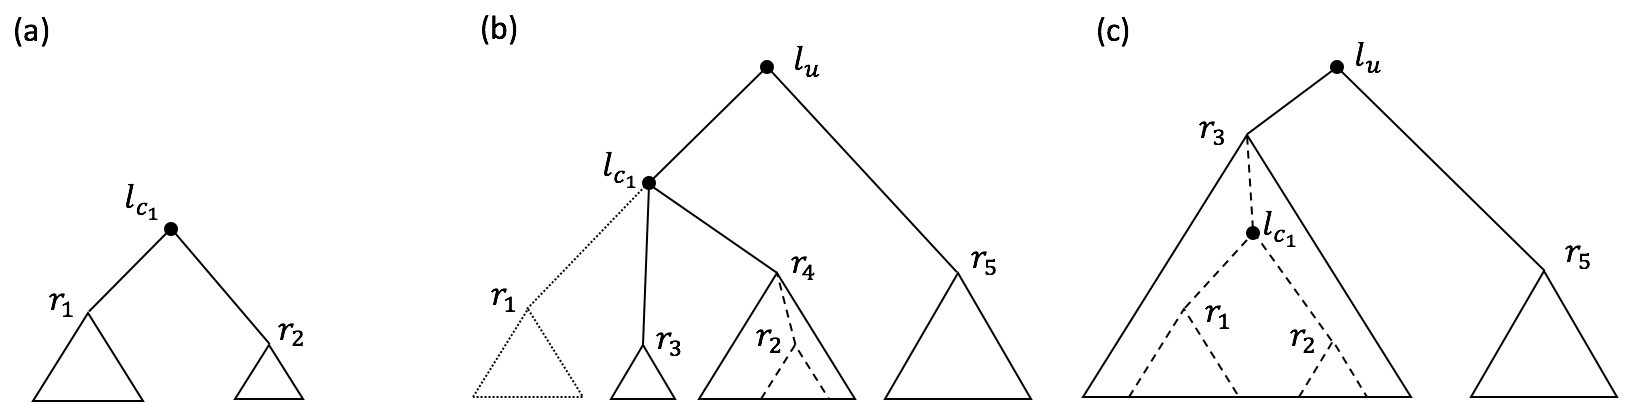
\includegraphics[scale=0.5]{incompatibilityrecursive}
        \centering
        \caption{Illustration of the recursive definition of $incompatible^{\TB}(u)$ using $incompatible^{\TB}(c_1)$, where $c_1 \in children(u)$. Note that $l_{c_1} = lca^{\TB}(\leafset(c_1))$ and $l_u = lca^{\TB}(\leafset(u))$. (a) shows only the portion of $\TB$ relevant to $c_1$. Here $RST^{\TB}(\leafset(c_1)) = \{r_1, r_2\}$. The triangles under these nodes represent the subtrees rooted at them. (b) shows a case where $l_{c_1} \in incompatible^{\TB}(u)$ and (c) shows a case where $l_{c_1} \not\in incompatible^{\TB}(u)$. In (b), $RST^{\TB}(\leafset(u)) = \{r_1, r_3, r_4, r_5\}$ while in (c), $RST^{\TB}(\leafset(u)) = \{r_6, r_7\}$. Nodes incompatible with $c_1$ are indicated by empty circles, while nodes incompatible with $u$ are indicated by squares.}
        \label{fig:incompatibilityrecursive}
    \end{figure}

    We demonstrate this result (proved below) in Figure~\ref{fig:incompatibilityrecursive}. Figure~\ref{fig:incompatibilityrecursive}(a) illustrates $incompatible^{\TB}(c_1)$. Here, $RST^{\TB}(c_1) = \{r_1, r_2\}$. The triangles under these nodes represent the subtrees rooted at them. The node $l_{c_1} = lca^{\TB}(\leafset^{\TA}(c_1))$. Then the nodes on the paths from $r_1$ and $r_2$ to $l_{c_1}$, indicated by empty circles, are incompatible with $c_1$, by Lemma~\ref{lem:incompatibilityrecursive}. Figure~\ref{fig:incompatibilityrecursive}(b) illustrates $incompatible^{\TB}(u)$. The node $l_u = lca^{\TB}(\leafset^{\TA}(u))$ and $RST^{\TB}(u) = \{r_1, r_3, r_4, r_5\}$. Observe that $r_4$ is a proper ancestor of $r_2$, $r_3$ is a proper descendant of $l_{c_1}$ and $r_5$ is not a descendant of $l_{c_1}$. Nodes in $incompatible^{\TB}(u)$ are indicated with squares, while nodes incompatible with $c_1$ remain marked with circles. Now nodes between $r_2$ and $r_4$, which were previously incompatible with $c_1$ are known to be compatible with $u$. Thus these must be removed from our set of candidates. However nodes between $r_4$ and $l_{c_1}$ should be kept. Further, all nodes between $r_3$ and $l_{c_1}$ were compatible with $c_1$, but are now known to be incompatible with $u$, by Lemma~\ref{lem:incompatibilityrecursive}. Nodes on the path from $r_1$ to $l_{c_1}$ were incompatible with $c_1$ and remain incompatible with $u$. We must also add nodes on the path from $r_5$ to $l_u$ to the set of incompatible nodes. Finally, we must also add nodes on the path from $l_{c_1}$ to $l_u$. However, this is not as clear cut as before. This is seen in Figure~\ref{fig:incompatibilityrecursive}(c), where $RST^{\TB}(u) = \{r_6, r_7\}$. Here, $r_6$ is an ancestor of $l_{c_1}$, in which case not all nodes between $l_{c_1}$ and $l_u$ are in $incompatible^{\TB}(u)$. Hence, we should only add nodes between $l_{c_1}$ and $l_u$ if there is some node $r \in RST^{\TB}(u)$ and $r \in RST^{\TB}(c_1)$.

    These observations are encapsulated as thus:
    \begin{itemize}
        \item For any node $r \in V(\TB)$, where $r \in RST^{\TB}(u)$ and $r \not\in RST^{\TB}(c_1)$, $path^{\TB}(r, l_u)$ needs to be added to our set of incompatible nodes.

        \item For any nodes $r, r' \in V(\TB)$, such that $r'$ is a proper ancestor of $r$, $r' \in RST^{\TB}(u)$ and $r \in RST^{\TB}(c_1)$, $path^{\TB}(r, r') \cup \{r'\}$ needs to be removed from our set of incompatible nodes. Note that this can be achieved by first removing $path^{\TB}(r, l_{c_1})$ and then adding back $path^{\TB}(r', l_{c_1})$. Further, the adding back part of this process is covered by the previous observation.

        \item It remains to ensure that $path^{\TB}(l_{c_1}, l_u) \cup \{l_{c_1}\}$ is added to the set. Recall, this will only be necessary if there is some node $r \in RST^{\TB}(u)$ and $r \in RST^{\TB}(c_1)$. If so, then we can simply add $path(r, l_u)$ to the set.
    \end{itemize}

    The three observations above motivated the definition of each of sets $newRST^{\TB}(u, c_1)$, $removedRST^{\TB}(u, c_1)$ and $oldRST^{\TB}(u, c_1)$ in Subsection~\ref{subsec:rootsofsubtrees}. With these in hand, we can go ahead and give a formal recursive formulation of $incompatible^{\TB}(u)$ in terms of $incompatible^{\TB}(c_1)$.
    \newline

    \begin{incompatibilityrecursive}
        \label{lem:incompatibilityrecursive}

        Given any trees $\TA$ and $\TB$, some internal node $u \in V(\TA)$ and $c_1 \in children(u)$, let $l_u = lca^{\TB}(\leafset(u))$ and $l_{c_1} = lca^{\TB}(\leafset(c_1))$, for any $r_1 \in oldRST^{\TB}(u, c_1)$ (if this does not exist then the relevant term below is empty),
        \begin{align*}
            incompatible^{\TB}(u) = &\left(incompatible^{\TB}(c_1)\ -\ \bigcup_{r \in removedRST^{\TB}(u, c_1)} path^{\TB}(r, l_{c_1})\right)\\
            &\cup\ \bigcup_{r \in newRST^{\TB}(u, c_1)} path^{\TB}(r, l_u)\\
            &\cup\ path^{\TB}(r_1, l_u)
        \end{align*}

        \begin{proof}
            First, it must be true that for any $r \in removedRST^{\TB}(u, c_1)$, there is some $r' \in newRST^{\TB}(u, c_1)$ such that $r'$ is a proper ancestor of $r$. If not, then since $\leafset^{\TB}(r) \subseteq \leafset^{\TB}(c_1) \subseteq \leafset^{\TA}(u)$ and there is no proper ancestor $r''$ of $r$ such that $\leafset^{\TB}(r'') \subseteq \leafset^{\TA}(u)$, $r \in RST^{\TB}(u)$. But then $r \not\in removedRST^{\TB}(u, c_1)$.

            $\longrightarrow$. Let $v \in incompatible^{\TB}(u)$. Then by Lemma~\ref{lem:incompatibilityrootsofsubtrees}, $v$ is a proper descendant of $l_u$. If there is some $r \in newRST^{\TB}(u, c_1)$ such that $v$ is a proper ancestor of $r$ then $v \in path^{\TB}(r, l_u)$. Otherwise, by Lemma~\ref{lem:incompatibilityrootsofsubtrees}, there must be some $r \in oldRST^{\TB}(u, c_1)$ such that $v$ is a proper ancestor of $r$. Then for all $r' \in removedRST^{\TB}(u, c_1)$, it cannot be that $v$ is a proper ancestor of $r'$. To see why, assume this is not true, i.e. there is some $r' \in removedRST^{\TB}(u, c_1)$ such that $v$ is a proper ancestor of $r'$. Then there is some $r'' \in newRST^{\TB}(u, c_1)$ such that $r''$ is a proper ancestor of $r'$. If $v$ is a descendant of $r''$, then $\leafset^{\TB}(v) \subseteq \leafset^{\TB}(r'') \subseteq \leafset^{\TA}(u)$. But then $v \not\in incompatible^{\TB}(u)$. Otherwise, if $v$ is a proper ancestor of $r''$, then there is some $r'' \in newRST^{\TB}(u, c_1)$ such that $v$ is a proper ancestor of $r''$, which contradicts our earlier assumption. Thus, if $v$ is a proper descendant of $l_{c_1}$, then $v \in incompatible^{\TB}(c_1)\ -\ \bigcup_{r \in removedRST^{\TB}(u, c_1)} path^{\TB}(r, l_{c_1})$. Otherwise, for any $r_1 \in oldRST^{\TB}(u, c_1)$, $v \in path^{\TB}(r_1, l_u)$ since $l_{c_1}$ is a proper ancestor of $r_1$ and a descendant of $l_u$.

            $\longleftarrow$. Let $v \in RHS$ of equation above.

            \textit{Case 1.} $v \in \bigcup_{r \in newRST^{\TB}(u, c_1)} path^{\TB}(r, l_u)$. Then by Lemma~\ref{lem:incompatibilityrootsofsubtrees}, $v \in incompatible^{\TB}(u)$.

            \textit{Case 2.} $v \in path^{\TB}(r_1, l_u)$. Since $r_1 \in RST^{\TB}(u)$, by Lemma~\ref{lem:incompatibilityrootsofsubtrees}, $v \in incompatible^{\TB}(u)$.

            \textit{Case 3.} $v \in incompatible^{\TB}(c_1)\ -\ \bigcup_{r \in removedRST^{\TB}(u, c_1)} path^{\TB}(r, l_{c_1})$ and\\[0.25em] % Overflows otherwise
            $v \not\in \bigcup_{r \in newRST^{\TB}(u, c_1)} path^{\TB}(r, l_u)$.\\[0.25em]
            Since $v \in incompatible^{\TB}(c_1)$, it is easy to see that $\leafset^{\TB}(v) \cap \leafset^{\TA}(u) \neq \emptyset$ and $\leafset^{\TA}(u) \not\subseteq \leafset^{\TB}(v)$. Also, there is some leaf $x \in \leafset^{\TB}(v)$ such that $x \not\in \leafset^{\TA}(c_1)$. If $x \in \leafset^{\TA}(u)$, then there is some $r \in RST^{\TB}(u)$ such that $r$ is an ancestor of $x$. Then $r \in newRST^{\TB}(u, c_1)$ since $x \in \leafset^{\TB}(r)$ and $x \not\in \leafset^{\TA}(c_1)$. We also note that $v$ is an ancestor of $x$. If $v$ is a proper ancestor of $r$, then $v \in path^{\TB}(r, l_u)$, which contradicts the definition of $v$. Thus $v$ is a descendant of $r$. Since $v \in incompatible^{\TB}(c_1)$, there is some $r' \in RST^{\TB}(c_1)$ such that $v$ is a proper ancestor of $r'$ (by Lemma 10). Then $r$ is a proper ancestor of $r'$, so $r' \not\in RST^{\TB}(u)$. Thus $r' \in removedRST^{\TB}(u, c_1)$. But then $v \in \bigcup_{r \in removedRST^{\TB}(u, c_1)} path^{\TB}(r, l_{c_1})$, which contradicts the definition of $v$. Thus $x \not\in \leafset^{\TA}(u)$ and so $v \in incompatible^{\TB}(u)$.
        \end{proof}
    \end{incompatibilityrecursive}

%    The above idea is the key insight that leads to an improvement in the runtime of \texttt{Filter\_Clusters}. As will be seen later, this property allows us to reduce the number of times we delete from a queue that maintains a subset of $V(\TB)$ from $O(n\,log\,n)$ to $O(n)$, thus decreasing total runtime from $O(n\,log^2n)$ to $O(n\,log\,n)$.

    \subsection{\texttt{Filter\_Clusters} algorithm}
    \label{subsec:filterclustersalgorithm}

    With this stricter definition of incompatibility in hand, we can work on a solution for \texttt{Filter\_Clusters}. We define a subroutine \texttt{Filter\_Clusters\_Helper} which, for some trees $\TA$ and $\TB$ where $\leafset^{\TA} = \leafset^{\TB}$, takes as input a subtree of $\TA$ (say $\TA[u]$) and $\TB$ and returns $RST^{\TB}(u)$. As a side effect, any node $u' \in V(\TA[u])$ is marked for deletion if $\weight(u') \leq max(\{\weight(C_1) : C_1 \in \mathcal{C}(\TB) \text{ and } C_1 \not\compatible \leafset^{\TA}(u')\})$. This means that any node in $\TA$ which is not more frequent that every cluster it is incompatible with in $\TB$ is marked for deletion. Then \texttt{Filter\_Clusters} uses \texttt{Filter\_Clusters\_Helper} as shown in Algorithm~\ref{alg:filterclusters}.

    \begin{algorithm}
        \caption{Filter\_Clusters}
        \label{alg:filterclusters}

        \begin{algorithmic}[1]
            \Input Trees $\TA$ and $\TB$ with $\leafset^{\TA} = \leafset^{\TB} = L$ where every cluster has a known $weight$.

            \Output A tree $T$ where $\mathcal{C}(T) = \{C : C \in \mathcal{C}(\TA) \text{ and } \weight(C) > max(\{\weight(C_1) : C_1 \in \mathcal{C}(\TB) \text{ and } C_1 \not\compatible C\})\}$ and $\leafset^T = L$

            \State Preprocess $\TB$ for $lca$ queries

            \State Do a bottom-up traversal of $\TB$ to compute $|children(v)|$ for all $v \in V(\TB)$

            \State Construct a cFL structure over $\TB$

            \State Construct an RMQ structure over $\TB$

            \State Let $T_{\alpha'} :=$ copy of $\TA$

            \State \texttt{Filter\_Clusters\_Helper}$(T_{\alpha'}, \TB)$

            \State Do a top-down traversal of $T_{\alpha'}$, deleting all marked nodes

            \State \Return $T_{\alpha'}$
        \end{algorithmic}
    \end{algorithm}

     \texttt{Filter\_Clusters\_Helper} decomposes $\TA$ into a \textit{centroid path} and a set of \textit{side trees} (similarly to \cite{jansson2018algorithms}). Observe that for any side tree $\tau \in \sigma(\TA)$, $|\leafset^\tau| \leq n/2$ and that $\{\leafset^{\TA}(u) : \tau \in \sigma(\TA)\}$ forms a partition of $L\, \backslash\, {p_1}$. We further note that for any internal node $p_i \in \pi(\TA)$, $\leafset^{\TA}(p_{i - 1}) \subset \leafset^{\TA}(p_i)$, i.e. the cluster associated with $p_{i-1}$ is a proper subset of $p_i$. This then leads to the intuition behind the procedure \texttt{Filter\_Clusters\_Helper} - recursively run the algorithm on the side trees, and then iterate over the centroid path from leaf to root. Here, for any non-leaf node $p_i \in \pi(\TA)$, we use \texttt{Compute\_Roots\_Of\_Subtrees} and Lemma~\ref{lem:incompatibilityrecursive}, to find $incompatible^{\TB}(p_i)$.

    A crucial part of this algorithm is the usage of a cFL structure and an RMQ structure on $\TB$ that allow us to query for the maximum weight of any node on the path between two given nodes (described in Sections~\ref{sec:cfd} and~\ref{sec:rmqtree}). This is because we do not actually need the set of incompatible nodes, we just need to find the largest weight over all incompatible nodes. Thus, rather than inserting all the nodes in say $path^{\TB}(v, v')$ into a set, we just insert $v$ indexed by $rmqTree^{\TB}[parent(v), childD(v, v')]$ (as obtained from the RMQ structure) into a priority queue. Notice that this plays well with Lemma~\ref{lem:incompatibilityrecursive}, which formulates incompatible nodes solely in terms of $path$. Thus, for convenience define, for any tree $\TB$ and nodes $v, v' \in V(\TB)$ where $v'$ is a proper ancestor of $v$, $rmqTree^{\TB}(v, v') = max_{w \in path^{\TB}(v, v')} \weight(w) = rmqTree^{\TB}[parent(v), childD(v, v')]$.

    We let $l_1$ be the leaf in $\TB$ labelled by $p_1$. The algorithm then initialises $roots$ to be $\{l_1\}$ and sets $counter(parent(l_1)) = 1$. Observe that the counter values are now correct with respect to the nodes in $RST^{\TB}(p_1)$ (as described in Lemma~\ref{lem:maintainingcounter}).

    It then uses Algorithm~\ref{alg:computerootsofsubtrees} and Lemma~\ref{lem:incompatibilityrecursive} to move up the centroid path, finding the nodes incompatible with $p_i \in \pi$. Thus, it first uses $RST^{\TB}(p_{i-1})$ and $boundary^{\TB}(p_i)$ to compute the sets $newRST^{\TB}(p_i, p_{i-1})$, $removedRST^{\TB}(p_i, p_{i-1})$ and $oldRST^{\TB}(p_i, p_{i-1})$. It is to facilitate this process that \texttt{Filter\_Clusters\_Helper} returns $RST^{\TB}(\leafset^{\TA})$ for the caller to use. These sets are used to compute $incompatible^{\TB}(p_i)$, after which we compare the largest weight in this set with the weight of $p_i$, and mark $p_i$ for deletion if its weight is not larger. Note that the counter values are inductively computed correctly since once we run \texttt{Compute\_Roots\_Of\_Subtrees} on $p_i$, the counter values are correct with respect to $RST^{\TB}(p_i)$, as laid out in Lemma~\ref{lem:maintainingcounter}.

    Finally, observe that at the end, the algorithm erases some counter values. Specifically, it erases the counters of the parents of nodes in $RST^{\TB}(\leafset^{\TA})$. This is because we do not want calls made to \texttt{Compute\_Roots\_Of\_Subtrees} for some $\tau_1 \in \sigma(\TA)$ to affect those made for a different $\tau_2 \in \sigma(\TA)$. Note that we do not need to erase any other counter values because nodes inside a maximal compatible subtree will never be encountered again while iterating upwards from some $boundary$.

    The procedure thus described is shown in Algorithm~\ref{alg:filterclustershelper}.

    \begin{algorithm}[H]
        \caption{Filter\_Clusters\_Helper}
        \label{alg:filterclustershelper}

        \begin{algorithmic}[1]
            \Input Trees $\TA$ and $\TB$ with $\leafset^{\TA} \subseteq \leafset^{\TB} = L$ where every cluster has a known $weight$.

            \Output $RST^{\TB}(\leafset^{\TA})$

            \SideEffect Marks any node $u \in V(\TA)$ for deletion iff $\weight(u) \leq \weight(v)$ for any $v \in V(\TB)$ with $u \not\compatible v$.

            \State Compute a centroid path $\pi = \langle p_{\gamma}, p_{\gamma - 1}, ..., p_1 \rangle$ of $\TA$, where $p_{\gamma}$ is the root of $\TA$ and $p_1$ is a leaf.

            \State \algorithmicforall\ side trees $\tau \in \sigma(\TA)$,
                associate \texttt{Filter\_Clusters\_Helper}$(\tau, \TB)$ with $\tau$

            \State Let $l_1 :=$ leaf in $\TB$ labelled by $p_1$

            \State $counter^{\TB}(parent(l_1)) := 1$

            \State $roots := \{l_1\}$

            \State $incompatible :=$ empty Brodal queue

            \For{$i := 2$ \textbf{to} $\gamma$}
                \State $boundary := \{\text{list of roots associated with } \tau : \tau \in \sigma(p_i)\}$

                \State $l_i := lca^{\TB}(l_{i-1} \cup boundary)$

                \State $new, removed, old :=$ \texttt{Compute\_Roots\_Of\_Subtrees}$(roots, boundary, \TB)$

                \State \algorithmicforall\ $r \in removed$, remove $r$ from $incompatible$
                \label{step:removedrootsremoval}

                \State \algorithmicforall\ $r \in new$, add $r, rmqTree^{\TB}(r, l_i)$ to $incompatible$

                \If{$old \neq \emptyset$}
                    \State Let $r \in old$

                    \State Remove $r$ from $incompatible$
                    \label{step:oldrootremoval}

                    \State Add $r, rmqTree^{\TB}(r, l_i)$ to $incompatible$
                \EndIf

                \IIEf{$incompatible$ is empty}
                    {$M := 0$}
                    $M :=$ maximum weight of a node in $incompatible$

                \IIf{$\weight(p_i) \leq M$}
                    mark $p_i$ for deletion

                \State $roots := old \cup new$
            \EndFor

            \State \algorithmicforall\ $r \in roots$, $counter^{\TB}(parent(r)) := 0$

            \State \Return $roots$
        \end{algorithmic}
    \end{algorithm}

    \bigskip
    \begin{filterclustersruntime}
        \label{lem:filterclustersruntime}

        The algorithm \texttt{Filter\_Clusters}$(\TA, \TB)$ runs in $O(n\,log\,n)$ time.

        \begin{proof}
            We preprocess $\TB$ for \textit{lca} queries using the technique of \cite{bender2000lca}. This takes $O(n)$ preprocessing time and thereafter allows us to answer \textit{lca} queries in $O(1)$ time. $\TB$ is also preprocessed to create the cFL and RMQ data structures using Lemma~\ref{lem:rmqdatastructure} and~\ref{lem:cfddatastructure}. These take $O(n\,log\,n)$ preprocessing time and thereafter allow us to answer $rmqTree$ queries in $O(1)$ time. The bottom-up traversal of $\TB$ to compute $|children(v)|$ for all $v \in V(\TB)$ takes $O(n)$ time. Finally, copying $\TA$ takes $O(n)$ time.

            As before, we use linked lists to implement sets of nodes, coupled with membership properties.

            The data structure used for $incompatible$ is the Brodal queue of \cite{brodal1995fast}. This allows $insert$ and $findMax$ operations in $O(1)$ time and $delete$ in $O(log\,m)$ time (where $m$ is the number of elements in the queue). Since the number of nodes in $\TB$ is $O(n)$, the number of elements in the queue is always $O(n)$ and so deletions cost $O(log\,n)$ time.

            Let $m = |\leafset^{\TA}|$ for some call to \texttt{Filter\_Clusters\_Helper}$(\TA, \TB)$. Recall that $n = |\leafset^{\TB}|$. Observe that for any cluster $C$, $|RST^{\TB}(C)| \leq |C|$. Thus $|boundary^{\TB}(p_i)| \leq |\leafset^{\TA}(p_i) - \leafset^{\TA}(p_{i-1})|$ and $\sum_{i = 2}^{\gamma} |boundary^{\TB}(p_i)| \leq m$. It can also be seen that $\sum_{P_i \in \mathcal{P}(\TA), p_j \in P_i} removedRST(p_j, p_{j-1}) \leq |V(\TA)|$.

            Computing the centroid path takes $O(m)$ time. Constructing the $boundary$ sets costs $O(m)$ time in total. Since $lca$ queries can be made in constant time and the total number of $lca$ queries is $O(m)$, this also costs $O(m)$ time.

            The runtime of \texttt{Compute\_Roots\_Of\_Subtrees} is $O(|boundary^{\TB}(p_i)| + |removedRST^{\TB}(p_i, p_{i-1})|)$. The cost due to the first half of this expression is $O(m)$. The cost due to the second half of this expression is $O(n)$ over all calls to \texttt{Filter\_Clusters\_Helper}.

            $O(m)$ insertions are made into $incompatible$, costing $O(m)$ time. Since the total size of all the removed sets is $O(n)$, there are a total of $O(n)$ deletions from $incompatible$ over all calls due to Step~\ref{step:removedrootsremoval}. Step~\ref{step:oldrootremoval} also causes a total of $O(n)$ deletions over all calls as this step happens once for each node in the centroid path, and every node in $\TA$ belongs to exactly one centroid path. Thus deletions cost a total of $O(n\,log\,n)$ time.

            We can hence write a recurrence for \texttt{Filter\_Clusters\_Helper} (ignoring steps that are being analysed over the entire call to \texttt{Filter\_Clusters}) in the following manner: $T(m) = \sum_{\tau \in \sigma(T)}T(|\leafset^{\tau}|) + O(m)$. Since for any $\tau \in \sigma(T)$, $|\leafset^{\tau}| \leq m/2$, there are $log\,m$ recursion levels, we get $T(n) = O(n\,log\,n)$.

            Finally, we note that it takes $O(n)$ time to process $T_{\alpha'}$ after \texttt{Filter\_Clusters\_Helper} is done. This is because deleting all marked nodes can be done in a top down traversal (using the \texttt{delete} operation described in Subsection~\ref{subsec:delete}), where every node's parent changes at most once. Further, recall that the total preprocessing time is $O(n\,log\,n)$ and the time set aside to be analysed over the entire call to \texttt{Filter\_Clusters} is $O(n\,log\,n)$. Thus, \texttt{Filter\_Clusters} runs in $O(n\,log\,n)$ time.
        \end{proof}
    \end{filterclustersruntime}

    \section{Constructing the FDCT}
    \label{sec:freqdiffconstruction}

    \begin{freqdiffruntime}
        \label{theorem:freqdiffruntime}

        Given a set $\mathcal{S}$ of $k$ trees with identical leafsets of size $n$, the algorithm \texttt{Frequency\_Difference}$(\mathcal{S})$ runs in $O(kn\,log\,n)$ time.

        \begin{proof}
            By Corollary~\ref{cor:freqdiffruntimecomponents} and Lemmas~\ref{lem:weightingruntime} and~\ref{lem:filterclustersruntime}, \texttt{Frequency\_Difference} runs in $O(kn\,log\,n + k \cdot n\,log\,n) = O(kn\,log\,n)$ time.
        \end{proof}
    \end{freqdiffruntime}

    \newpage
    \bibliographystyle{plain}
    \bibliography{interim_report}
\end{document}
